% !TEX root = ../These_Robin_Master.tex
\setcounter{chapter}{5}
\graphicspath{{chap6/}}

\chapter{Retours sur la co-construction et l'exploration d'un modèle en situation d'interdisciplinarité}
\label{chap:chap6}
%\vspace*{-2.5em}
%\begin{center}
%	{\large \hl{Version 2020-01-03}}
%\end{center}
%\vspace*{-1em}
%\begin{itemize}
%	\item 26/09/2019 : fin 6.1 + envoi à Lena
%	\item 07/12/2019 : début 6.2
%	\item 11/12/2019 : fin 6.2 + envoi à Lena
%	\item 03/01/2020 : recopie du Google Docs validé par Lena, Lucie et Julie
%\end{itemize} 
%\vspace*{-1em}
\setcounter{minitocdepth}{2}
\vfill
\setstretch{1.5}
\minitoc
\setstretch{1.1}
\clearpage
\phantomsection

\section*{Introduction}
\addcontentsline{toc}{section}{\protect\numberline{}Introduction}

Dans les chapitres précédents, les approches suivies pour la co-construction et l'évaluation du modèle \simfeodal{} ont été décrites.
Il me semble, en accord avec le positionnement exposé dans le \cref{chap:chap1}, que cette démarche est porteuse quand elle est effectuée de manière véritablement collective et interdisciplinaire.
Dans le cas du groupe de travail constitué autour de \simfeodal{}, cette démarche s'est révélée fructueuse.
Dans le présent chapitre, je reviendrai de manière réflexive sur cette expérience de modélisation interdisciplinaire.
Ce retour critique permettra d'en faire émerger les atouts, les difficultés, mais aussi d'y discerner les particularités, liées à ce modèle spécifique, vis-à-vis du cadre plus générique de la modélisation.
La diversité des points de vue présentés dans cette thèse -- conceptuel, théorique, méthodologique ou encore technique -- me paraît devoir être mobilisée à nouveau au sein de ce retour global sur une expérience collective inscrite dans la longue durée.

On a plusieurs fois insisté, notamment dans le \cref{chap:chap3}, sur le fait qu'il est difficile de séparer chronologiquement la construction et le paramétrage d'un modèle d'une part, et son évaluation et son exploration d'autre part.
Ces tâches s'inscrivent en effet dans une spirale d'allers-retours constants.
La discrétisation de ce continuum est forcément artificielle mais nécessaire pour le décrire de manière linéaire au sein d'une narration.
Dans cette thèse, cette narration a ainsi été rectiligne, présentant d'abord le modèle, son évolution, puis la méthodologie mise en place pour l'évaluer et l'explorer, autour du cadre théorique des \textit{(geo)visual analytics}.


Au sein de ce chapitre, j'ai choisi d'inverser cet ordre en présentant d'abord les retours liés à l'exploration visuelle des données de simulation, et, seulement ensuite les retours plus conceptuels sur le processus de co-construction interdisciplinaire d'un modèle.
Cette inversion s'explique par la prépondérance qui a été accordée à la visualisation des données dans le processus d'ensemble qu'a été la construction de ce modèle.
L'approche visuelle me paraît être tout à la fois une interface disciplinaire efficace et une condition préalable indispensable à l'expérience de modélisation collective, qui plus est interdisciplinaire et caractérisée par une forte hétérogénéité de cultures scientifiques.

\clearpage
\let\orisectionmark\sectionmark
\renewcommand\sectionmark[1]{}%
\section{L'analyse exploratoire de données issues de simulation, une approche aux possibilités multiples\label{sec:retour-eda}}
\orisectionmark{Retour sur l'analyse de données de simulation}
\let\sectionmark\orisectionmark

L'évaluation des données issues de \simfeodal{} a été inscrite dans plusieurs cadres méthodologiques :
	la visualisation de données (\textit{InfoVis}), l'analyse exploratoire de données (\textit{EDA}) et les \textit{(geo)visual analytics} d'une part, mais aussi d'autre part, la démarche de face validation et d'évaluation visuelle défendue dans les \cref{chap:chap3,chap:chap5}.
Les premiers cadres sont utilisables avec toutes les données numériques, y compris spatio-temporelles, à l'instar des données de sortie de \simfeodal{}.
Les seconds tiennent plus à la démarche de modélisation, qu'il s'agisse de simulation, de modélisation statistique ou mathématique, etc.
Il me semble important, dans cette partie de revenir sur le cas spécifique de la visualisation et de l'exploration de données issues de simulation, notamment au regard de l'analyse exploratoire de données empiriques plus classiques.
Une fois ces spécificités isolées, on appréhendera plus globalement le rôle et l'importance de la visualisation de données dans le cadre de la modélisation.
Une dernière sous-partie explorera les différentes pistes possibles d'utilisation de l'exploration visuelle des sorties de modèle, en cherchant à passer de l'exploration à la validation de modèles de simulation\footnote{
	Toute cette partie (\cref{sec:retour-eda}) s'appuie sur un chapitre d'ouvrage en cours de publication \autocite{cura_visualisation_2020}.
	Il est consacré au rôle et aux méthodes de la visualisation dans le domaine de la modélisation géographique.
	Moins synthétique que la présente partie, ce chapitre d'ouvrage peut en offrir un complément utile.
}.



\subsection{L'analyse exploratoire de données, un cadre théorique et méthodologique adapté à l'exploration de toutes les données spatiales et spatio-temporelles \label{subsec:genericite-donnees-simul}}

Le \cref{chap:chap4} et particulièrement la présentation de la démarche d'exploration visuelle des données issues de sorties de simulations (\cref{sec:explorer-sorties-simfeodal}) pourrait tout à fait s'appliquer à des données plus classiques.
La problématique des données hétérogènes, liées par un Modèle Conceptuel de Données adapté, explorées en multipliant les angles de vue, n'est en effet pas spécifique aux données de simulation.
Toutefois, plusieurs aspects de la simulation, et en particulier l'évolutivité des données et la dimension réplicative, contraignent l'exploration visuelle et forcent à abandonner certaines méthodes traditionnelles de représentation graphique.
Dans cette sous-partie, nous revenons sur la place des données issues de simulation dans le panorama des types de données, et nous montrons que l'analyse exploratoire de données peut tout à fait être appliquée à ces dernières, en posant quelques contraintes supplémentaires.

\paragraph{Parallèles entre exploration de données et exploration de modèle.}
Avant tout, il faut rappeler que l'exploration des données de sortie d'un modèle de simulation est une manière d'explorer le modèle de simulation en lui-même (voir \cref{subsec:apports-analyse-visuelle-sensib}).
Par exploration, on entend ici une recherche de compréhension des logiques de fonctionnement du modèle, c'est-à-dire des effets produits par les interactions complexes entre les agents et entre les mécanismes du modèle.
L'exploration d'un modèle s'inscrit ainsi dans un parallèle très net avec l'analyse exploratoire de données (EDA).
Les deux démarches sont en effet largement semblables, et contiennent les mêmes étapes.

En premier lieu, l'exploration de données et l'exploration de modèles cherchent à repérer les structures globales présentes dans les données (et modèles).
Dans le premier cas, il s'agit de dégager des tendances générales depuis un jeu de données.
Cela peut passer par des analyses de corrélations, par l'étude de variations des amplitudes, par la caractérisation des évolutions temporelles, etc.
Pour les modèles, on cherche également, d'abord, à observer les grandes dynamiques produites par le modèle de simulation, la forme de l'évolution temporelle de ces dynamiques, les effets de rétro-action les plus visibles, etc.
Explorer un modèle, c'est ainsi et avant tout comprendre les effets croisés des mécanismes sur la structure globale, agrégée, des entités modélisées.

En second lieu, l'exploration de données peut se faire par des analyses plus fines, en cherchant par exemple à discerner des groupes d'unités aux comportements différents, des \textit{outliers}, des variables aux relations inattendues, etc.
En sciences humaines et sociales, ce moment de l'analyse est souvent l'occasion d'étudier les résidus de modèles statistiques afin d'entrer dans une caractérisation plus fine des particularités de certaines entités, spatiales ou non.
La démarche est là encore la même que dans l'exploration de modèles :
	après avoir dégagé les tendances générales, on peut changer d'échelle d'observation, en observant par exemple le comportement individuel de certains agents, ou en faisant varier plus finement certains paramètres pour en observer les influences sur le déroulé de la simulation.
Là encore, la première phase d'étude, agrégée, intervient comme un filtre ou un modèle nul, dont on cherche ensuite à caractériser les écarts ou la composition désagrégée.
Dans le chapitre précédent, l'analyse de sensibilité illustrait assez largement cette démarche.
La première phase de filtrage des paramètres permettait notamment de mettre en évidence les co-variations habituelles des indicateurs de sortie selon les valeurs de paramètres mobilisées.
La seconde phase d'analyse visuelle, plus précise, permettait d'étudier plus avant le détail de ces variations, et même de mettre en évidence des co-variations inverses à celles de la majorité des cas (voir l'exemple du paramètre de pondération de la création de nouvelles paroisses dans les agrégats, \cref{sssec:sensib-params-eglises}).

Les démarches d'analyse exploratoire de données et de modèles sont donc très similaires, reposant sur les mêmes méthodes appliquées à des objets différents.
Dans les deux cas, les éléments observés sont en définitive des données numériques multi-variées, qui constituent des proxy de phénomènes sociaux et/ou spatiaux dans le premier cas, et des proxy des dynamiques modélisées dans le second.

\paragraph{Les données issues de simulation, des données spatio-temporelles \og intermédiaires\fg{}.}
En informatique, il est classique de différencier les types de bases de données selon leur \og taille\fg{} ou la masse des données contenues, c'est-à-dire selon le nombre d'entités/lignes représentées ou selon l'espace disque effectivement occupé pour les stocker.
Les données de faible taille et poids sont très répandues, et peuvent être traitées avec l'ensemble des solutions logicielles classiques existantes, voire à la main pour les plus ténues (régions françaises par exemple).
À l'opposé, les \og \textit{big data}\fg{} représentent des données qui ne peuvent ni être stockées ni être traitées sur un ordinateur personnel classique et requièrent dès lors de faire appel à des technologies informatiques avancées.
Entre ces deux extrêmes, j'introduis le terme de \og données intermédiaires\fg{} pour désigner les données trop larges pour être traitées avec les solutions classiques, mais trop restreintes pour justifier l'emploi des techniques complexes associées au \textit{big data}.
Le \cref{tab:donnees-intermediaires} exemplifie l'éventail de données qui existe entre ces deux extrêmes.

\begin{table}[H]
	\centering
	\resizebox{\textwidth}{!}{%
	{\renewcommand{\arraystretch}{1.1}%
		\begin{tabular}{|M{2.25cm}|M{2cm}|M{4.5cm}|M{3.25cm}|M{4.25cm}|M{1cm}|}
			\hline
			\multicolumn{3}{|c|}{\textbf{Données}} & \multicolumn{2}{c|}{\textbf{Stockage et analyse}} & \\ \hline
			\textbf{Quantité} & \textbf{Espace disque} & \textbf{Exemples} & \textbf{Type de stockage} & \textbf{Outils d'analyse} & \textbf{Type}\\ \hline
			$\le$ 1 000 lignes & $\sim$ 1 Mo & Données de recensement agrégé & \multirow{2}{*}{Fichiers textes} & \multirow{2}{*}{\makecell{Traitement manuel,\\tableurs, SIG\ldots}} & \parbox[t]{2mm}{\multirow{3}{*}{\rotatebox[origin=c]{-90}{Données classiques}}} \\ \cline{1-3} 
			1 000 - 100 000 lignes & $\sim$ 1-50 Mo & Recensement détaillé & & & \\ \cline{1-5} 
			100 000 -- quelques millions de lignes & $\sim$50 Mo -- 1 Go & Données individuelles, séries temporelles de capteurs multiples\ldots & Tableur ou fichier binaire (Shapefile, geopackage...) & Outils statistiques interactifs (\textit{GUI}) ou en lignes de commande (\textit{CLI}) & \\ \hline
			\rowcolor[HTML]{E8E8E8} 10 à 100 millions de lignes & $\sim$1 - 10 Go & Jeux de données \textit{opendata} récents: équipements, contenu généré par les utilisateurs (tweets), \textit{VGI}\ldots & Systèmes de Gestion de Bases de Données (SGBD) & CLI (R/Python) via SQL, OLAP\ldots & \parbox[t]{10mm}{\rotatebox[origin=c]{-90}{\makecell{Données \\intermédiaires}}} \\ \hline
			\textgreater 100 millions de lignes & \textgreater 10 Go & Données spatio-temporelle à résolution fine, collecte automatisée de capteurs, jeux de données des grosses entreprises du numérique\ldots & SGBD distribués & Calcul intensif (\textit{High-Performance Computing}) & \parbox[t]{2mm}{\rotatebox[origin=c]{-90}{\textit{Big data}}} \\ \hline
	\end{tabular}}}
	\caption[Caractérisation des donnés intermédiaires dans le spectre des donnés.]{Caractérisation des donnés intermédiaires dans le spectre des donnés. Adapté de \textcite{cura:halshs-02290556}}.
	\label{tab:donnees-intermediaires}
\end{table}

Dans la ligne grisée, les données sont trop massives pour être traitées de manière classique mais demeurent contenues dans des volumes informatiques que l'on est souvent amenés à manipuler (fichiers de films, logiciels, etc.).
Ce sont ces données que l'on peut nommer \og données intermédiaires\fg{}.
Elles sont d'une taille largement praticable, mais posent déjà des obstacles techniques difficiles à franchir sans faire appel à des méthodes d'archivage et d'analyse de données récentes.

Ce tableau peut facilement être comparé au \cref{tab:tab-accroissement}, qui figure la massification des données issues de simulation au fur et à mesure de l'exploration d'un modèle.
Ces dernières s'inscrivent tout à fait dans les mêmes problématiques que les \og données intermédiaires\fg{}.
Les données issues de simulation ne sont pas des \textit{big data} car elles ne sont ni véloces, ni variables ou imprévisibles, mais leur masse requiert tout de même des outils adaptés, tant pour leur archivage que pour leur interrogation.
Les solutions mises en place pour leur analyse (\cref{chap:chap4}) sont précisément des solutions pensées pour ces données intermédiaires, où les infrastructures de type \og bases de données analytiques\fg{} se révèlent particulièrement efficaces.

\paragraph{Quelles spécificités des données de simulation ?}\label{par:specificites-donnees-simul}
Les données issues de simulation peuvent être vues comme des données intermédiaires, mais elles s'en distinguent toutefois -- notamment vis-à-vis du caractère empirique des exemples données dans le \cref{tab:donnees-intermediaires} -- par un certain nombre de spécificités qui complexifient leur analyse et requièrent le développement ou au moins l'usage d'outils particuliers, tels qu'illustrés dans le \cref{chap:chap4}.

Au regard de certaines spécificités, on pourrait par exemple être tenté de classer ces données issues de simulation dans les \textit{big data} plutôt que dans les données intermédiaires.
Certes, contrairement aux \textit{big data}, les données issues de simulation ne sont par essence ni incomplètes, ni hétérogènes, puisqu'elles sont générées directement par le modélisateur.
Cependant, dans le cas d'un modèle conçu et développé dans la durée, les problématiques y sont assimilables :
	le modèle évolue et les données qu'il est en mesure de générer évoluent concomitamment.
En dépit d'un contrôle complet sur la chaîne de production de données, les données issues d'expériences successives de simulation peuvent ainsi poser des problèmes d'hétérogénéité, tels qu'illustrés dans la \cref{subsec:organiser-indicateurs-rapports} (p.~\cpageref{par:compatibilites-generations}).

Une autre spécificité, cette fois-ci due à la nature des modèles de simulation plus qu'à leur usage, tient à leur essence souvent stochastique.
Pour analyser le comportement simulé par un modèle, il est ainsi nécessaire de prendre en compte plusieurs simulations différentes, caractérisées par un même jeu de valeurs de paramètres, mais dont l'aléa aura varié entre ces \og réplications\fg{}.
Pour caractériser le comportement du modèle sur chacun des indicateurs de sortie de simulation produits, il est alors indispensable de procéder à des opérations de résumé statistique (moyenne, valeurs extrêmes, etc.) sur des \og agrégations\fg{} de simulations, agrégations qui sont aussi nécessaires pour la visualisation graphique de ces indicateurs.
Pour les données temporelles, on peut utiliser des représentations graphiques de dispersion, tels que les \textit{box-plots} largement employés dans ce travail.


Quant à la dimension spatiale, des typologies des opérations d'agrégations et de résumés statistiques de données spatio-temporelles existent (\cite{bach_review_2014} utilisent le terme de \og \textit{flattening}\fg{} pour les définir), mais leur mise en place est peu aisée et tend à s'appliquer à des outils \textit{ad hoc} plus qu'à des modèles génériques.
Le logiciel \textsc{VisuAgent} \autocite{cura_visuagent_2014} (\cref{subfig:visuagent}) constitue un exemple d'une telle plateforme \textit{ad hoc}, attachée aux données du modèle de colonisation d'un espace vide \og HU.M.E\fg{} \autocite{lenechet:hal-02025441}, dont elle cherchait à faciliter l'exploration.
L'ambition de la plateforme \textsc{VisuAgent} était d'explorer une diversité de méthodes de résumé (observer les valeurs extrêmes ou des indicateurs de dispersion plutôt que des valeurs centrales par exemple) et de rendu (représentations basées sur les combinaisons possible de l'espace, du temps et de l'agrégation de simulations) plutôt que de construire des indicateurs habituels d'évolution (spatio-)temporels.

\begin{figure}[H]
	\centering
	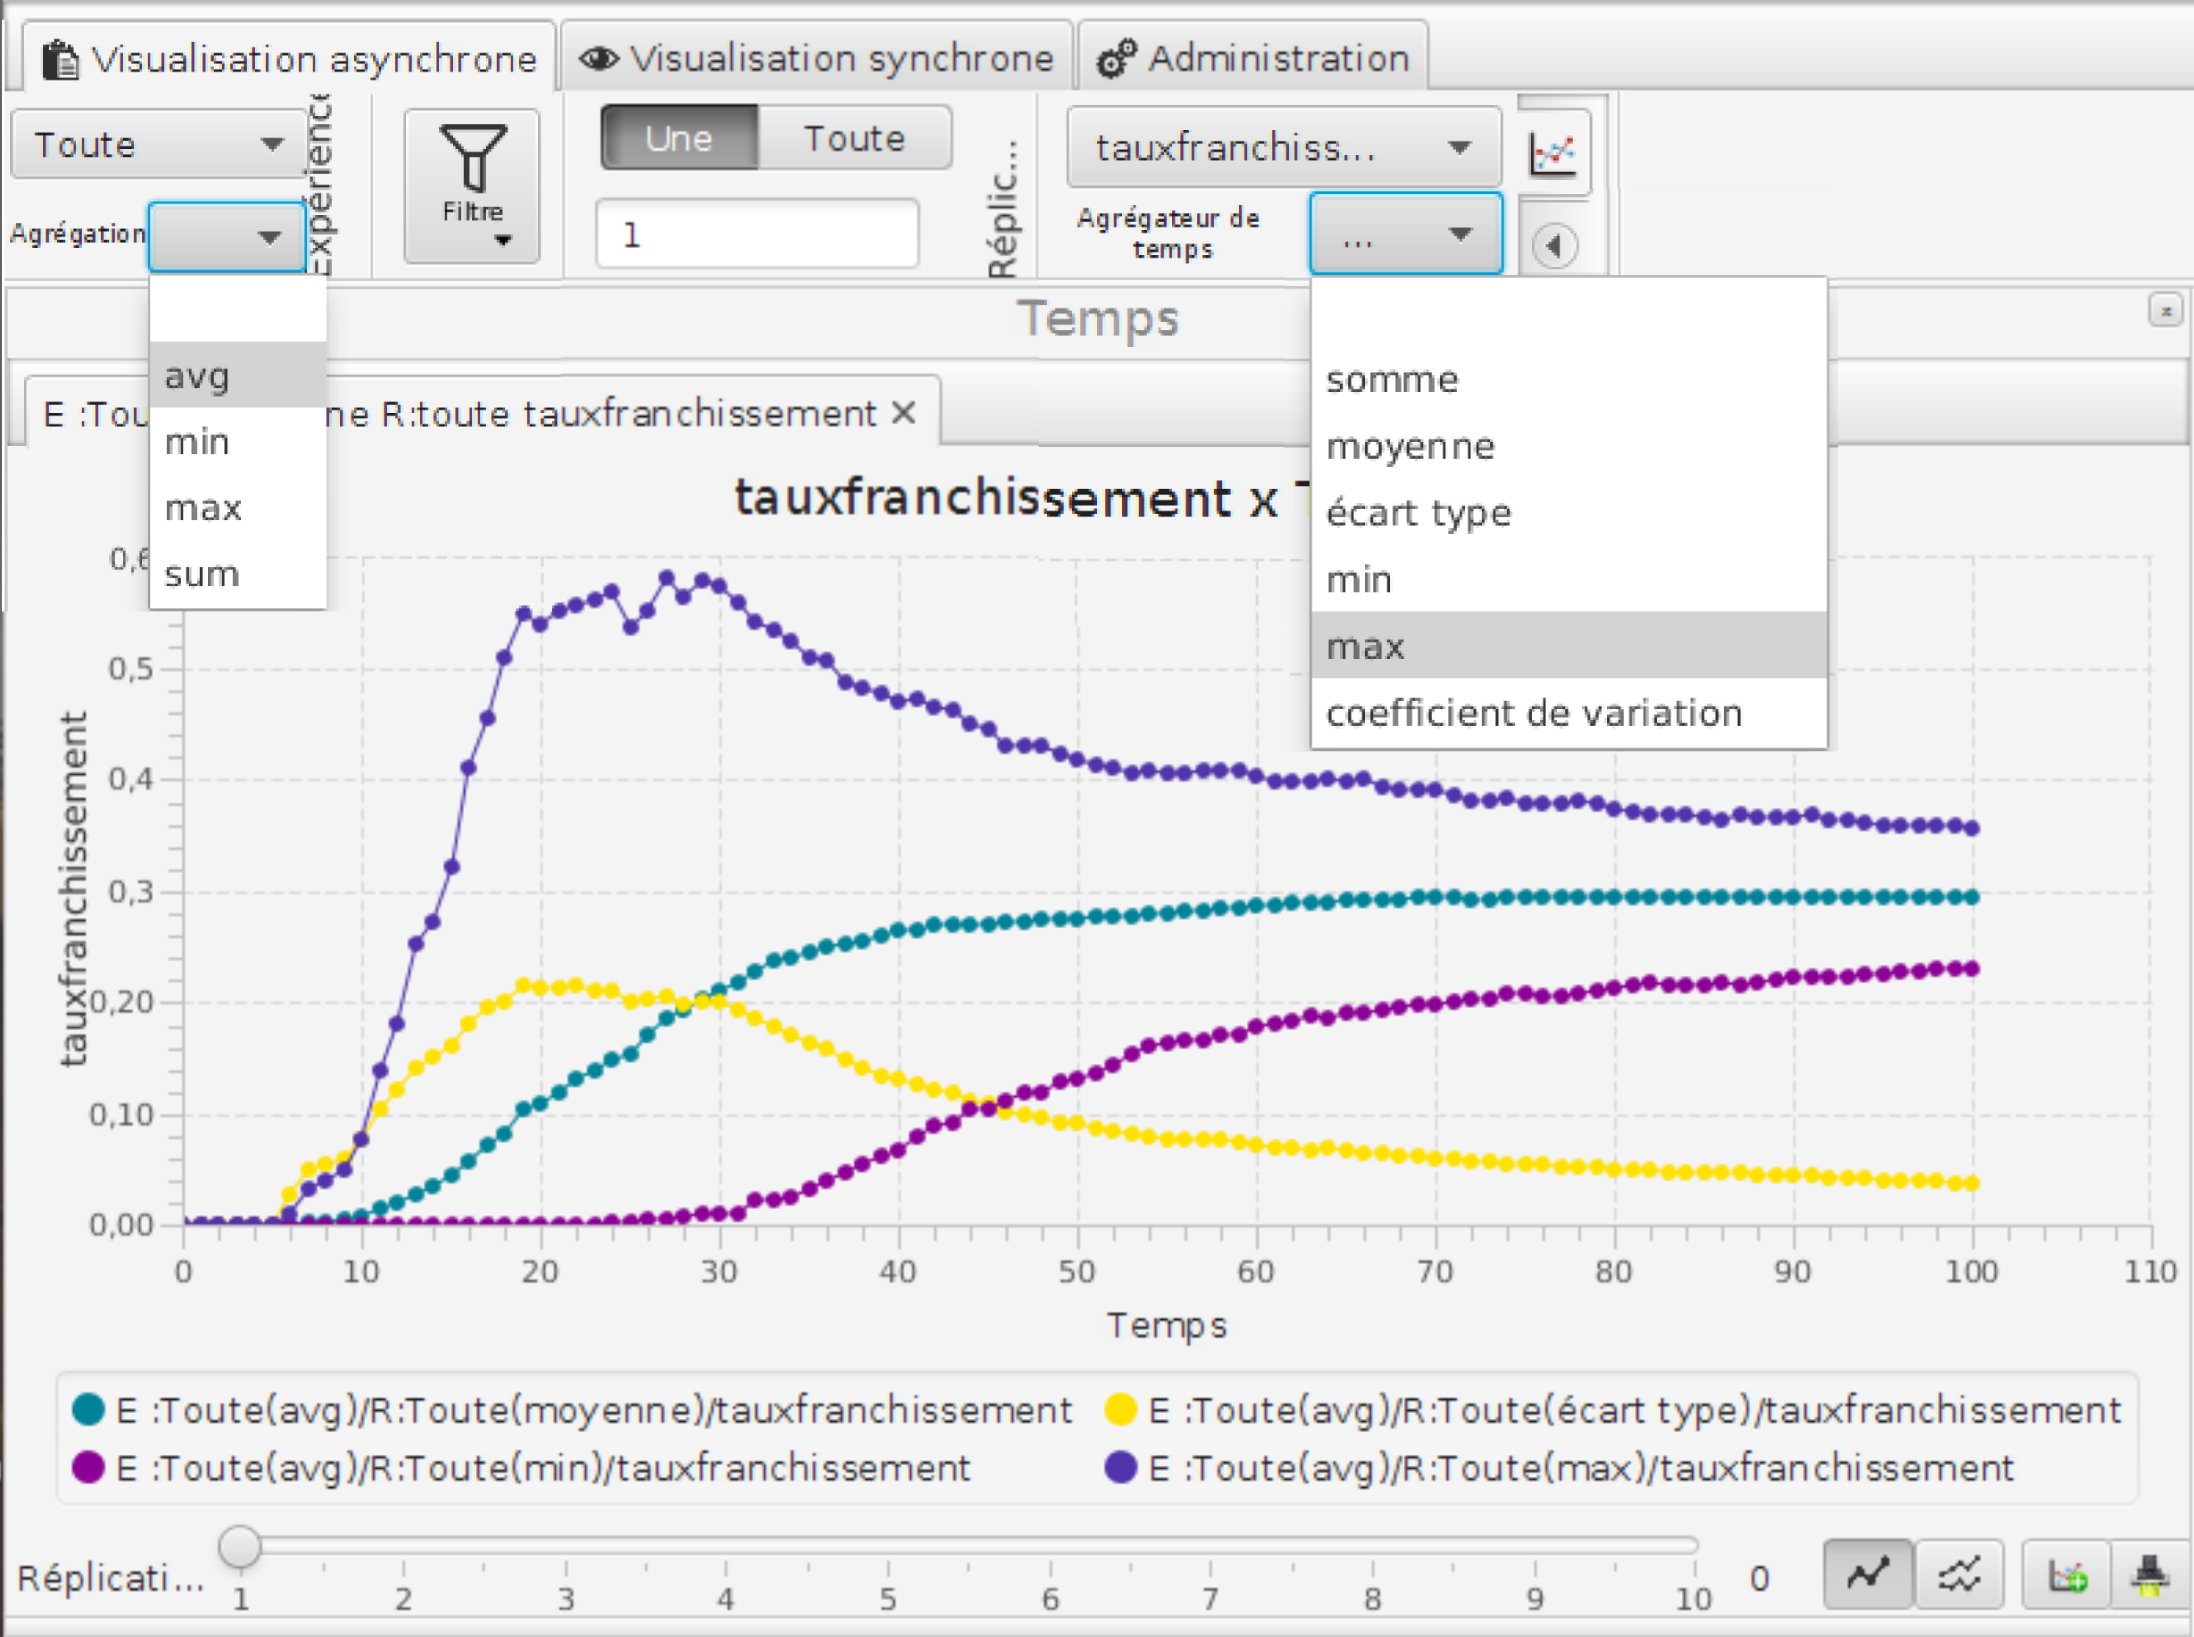
\includegraphics[width=\linewidth]{img/visuagent_agregations.png}
	\caption{Visualisation de différentes méthodes de résumés statistiques, sur les dimensions réplicatives et temporelles, avec le logiciel \textsc{VisuAgent}.}
	\label{subfig:visuagent}
\end{figure}


Dans le cadre de données de simulation, et en particulier quand l'espace est continu\footnote{
	Pour les données spatiales discrètes, par exemple quand l'espace prend la forme de cellules ou d'un maillage établi (régions, états, etc.), on peut mettre en place des systèmes graphiques de représentation de la forme des distributions d'une variable.
	Voir \textcite{ribecca_chart_2018} par exemple.	
}, on ne peut réaliser d'agrégations des données sur la dimension spatiale que dans le cas où celle-ci est stable, c'est-à-dire que les données agrégées sont directement assimilables les unes aux autres.
Dans un modèle comme \simfeodal{}, l'agrégation n'est pas possible car la répartition spatiale des agrégats, châteaux et églises change à chaque simulation (voir \cref{chap:chap2}, \cref{sec:initialisation}).
La \cref{subfig:agreg-espace} illustre ce problème en présentant deux sorties théoriques de simulation, très proches en termes d'évolution, d'espacement, de structure globale, mais dont on ne peut tirer une représentation synthétique de manière classique puisque cela reviendrait à \og créer\fg{} des positions moyenne d'objets qui ne sont pas assimilables et n'ont que peu de sens thématiquement.
Pour le modélisateur, deux alternatives sont possibles.
Ou bien l'on se contente d'indicateurs synthétiques numériques classiques, agrégeables, mais qui ne rendront pas correctement compte de la situation spatiale, ou bien l'on mène une observation de chacune des cartes correspondant aux différentes données produites par les réplications.

\begin{figure}[H]
	\centering
	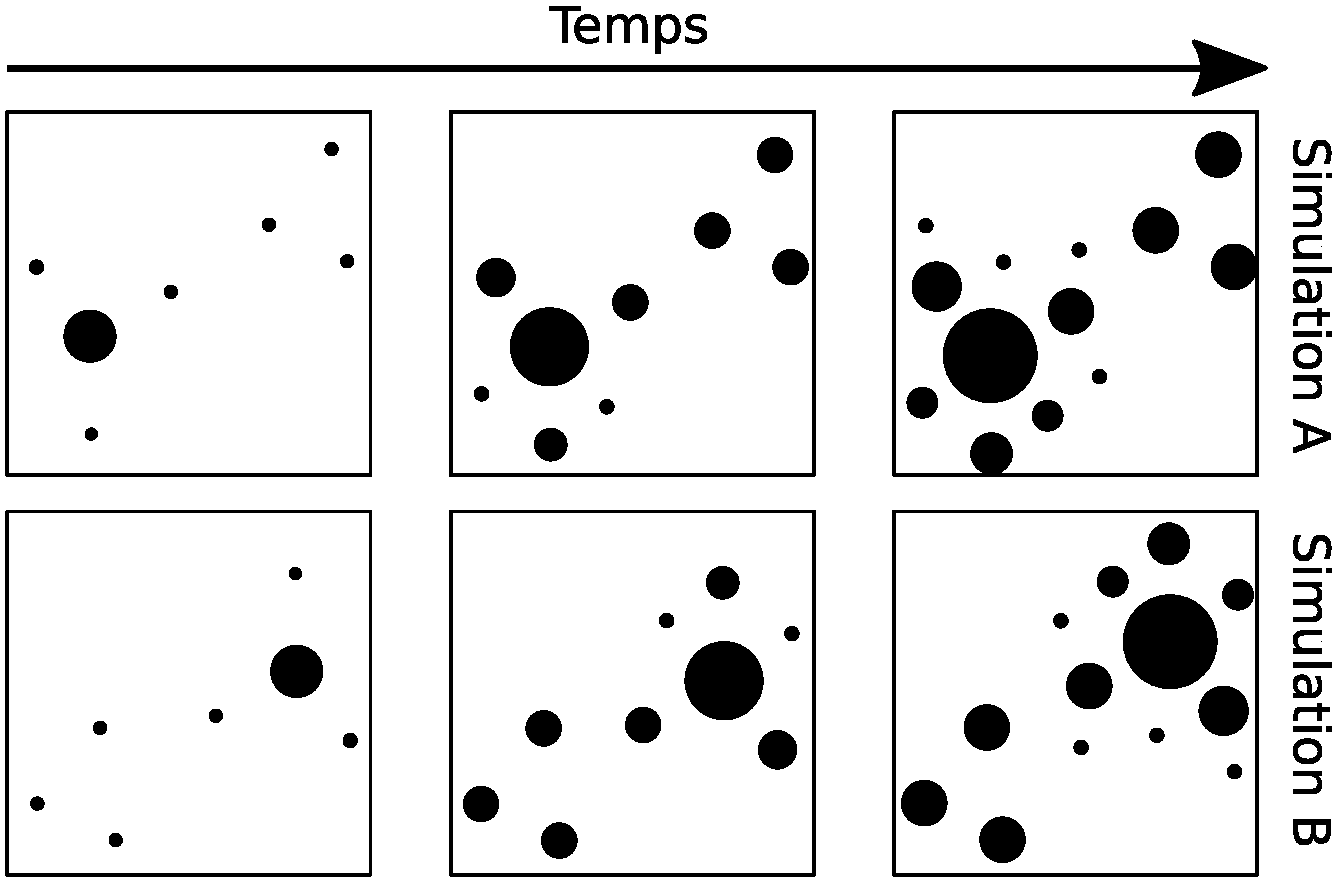
\includegraphics[width=.8\linewidth]{img/espace_theoriques.pdf}
	\caption[Deux cas théoriques d'évolution spatio-temporelle très similaires mais non agrégables.]{Deux cas théoriques d'évolution spatio-temporelle très similaires mais non agrégables. Exemples tiré de \textcite{cura_visualisation_2020} }
	\label{subfig:agreg-espace}
\end{figure}


\subsection{Construction de connaissances par l'exploration visuelle d'un modèle \label{subsec:construction-connaissance-explo}}


Dans son Habilitation à Diriger des Recherches, \citeauteur{banos_pour_2013} décrivait neufs \og principes forts\fg{} de la modélisation \autocite[76--84]{banos_pour_2013}.
Dans \textcite{cura_visualisation_2020}, je mène une comparaison point à point de ces neufs principes en les appliquant à la visualisation de données issues de modèles.
Je reprendrai ici quelques uns des arguments qui me paraissent importants, en termes de réflexivité, sur les gains de connaissances que l'exploration visuelle d'un modèle peut apporter.

\paragraph{La visualisation de modèle comme outil d'interdisciplinarité.}
Les modélisateurs savent l'importance du dialogue dans la construction d'un modèle.
Dans son principe 2, \textcite[77]{banos_pour_2013} l'explicite ainsi :
	\og Le modélisateur doit avoir conscience du caractère fondamentalement limité de ses compétences.
	Ce qui peut être perçu comme une faiblesse est pour moi une force.
	Assumée, cette réalité mène naturellement à la collaboration.
	De manière très générale, je dirais même que modéliser un système complexe est un acte par essence collaboratif\fg{}.

La visualisation est un outil de communication au service de la transmission et de la diffusion d'un message.
Sans prise en compte de sa réception par ses lecteurs, le risque est important de concevoir un média peu compréhensible et donc peu utile.
Les retours du public visé sont donc importants, d'autant plus quand la visualisation doit aider à appuyer ou à transmettre un message complexe, requérant une expertise thématique, comme c'est souvent le cas dans le cadre d'un projet de modélisation.
Dès lors, le visualisateur ne peut agir seul, de la même manière que le modélisateur ne peut se contenter de sa seule expertise.

C'est d'autant plus vrai dans le cadre d'un modèle co-construit en interdisciplinarité.
Les différences de culture scientifique s'expriment aussi en termes de \og culture des données\fg{} (\textit{data litteracy}), c'est-à-dire par des habitudes et compétences hétérogènes en matière d'analyse et de visualisation de données.
Explorer visuellement un modèle, c'est avant tout se mettre d'accord sur ce que l'on veut observer, et ensuite sur la manière de le représenter.
Cette démarche, obligatoire, force à l'explicitation des détails techniques du modèle implémenté et de la manière dont les indicateurs de sortie sont obtenus, afin de minimiser le risque d'erreurs d'interprétation.

Par cette explicitation, l'exploration visuelle d'un modèle force à la collaboration et, dans un cadre interdisciplinaire, à un réel partage de connaissances et de pratiques.
Ce faisant, l'exploration visuelle d'un modèle participe largement au rôle d'interface disciplinaire que la modélisation, en tant que telle, endosse.

\paragraph{L'exploration visuelle comme modélisation.}
Simulation et visualisation sont des domaines scientifiques étudiés par des communautés disciplinaires différentes et peu interconnectées.
Au sein même des réseaux francophones, les géographes se partagent par exemple entre différentes communautés.
La communauté de la géographie théorique et quantitative (colloques ThéoQuant et ECTQG, réseau S4, liens avec les Instituts des Systèmes Complexes, etc.) conçoit et développe des modèles depuis de nombreuses années, mais aussi des outils pour en explorer les sorties (voir \textcite{tannier:halshs-01003259} par exemple).
D'un autre côté, la communauté géomatique (colloques SAGEO, GDR CASSINI/MAGIS, etc.) s'intéresse notamment à l'exploration de données spatio-temporelles, à leur visualisation et leur modélisation, avec peut-être une entrée plus méthodologique et technique que le premier ensemble.
Ces deux communautés communiquent peu, et cette situation n'est pas nouvelle\footnote{
	Il suffit de lire l'article qui introduit la publication des actes du colloque SAGEO 2005 pour s'en convaincre \autocite{josselin_presentation_2006}.
}.

Pourtant, dans les faits, la représentation graphique telle qu'elle est utilisée et théorisée en géographie théorique et quantitative, et notamment la cartographie qui a un rôle central\footnote{
	Par exemple chez \textcite[246--247]{pinchemel_geographie_1979}, pour qui \og seule la représentation cartographique fait ressortir les organisations géographiques, les structures et les systèmes géographiques.
	La carte, le langage cartographique apparaissent aussi comme l'expression, comme le révélateur privilégiés de la géographie.
	La pensée géographique se lit dans les représentations cartographiques\fg{}.
}, peut largement être considérée comme une forme de modélisation des phénomènes sociaux et spatiaux\footnote{
	À l'instar de la \og modélisation graphique\fg{}, ou chorématique de \textcite{brunet1980composition}.
} au regard des définitions d'un modèle que nous avons adoptées dans cette thèse\footnote{
	Voir par exemple la définition de \textcite{minsky_matter_1965}, citée dans l'\cref{chap:intro}.	
}.
L'exploration visuelle, composée d'une succession de compositions graphiques que l'on raffine, que l'on transforme et dont on change le point de vue, est alors en tout point similaire au processus de construction d'un modèle de simulation \autocite{andrienko2018viewing}.
L'exploration visuelle n'est donc pas un processus isolé, particulier, et peut alors s'inscrire dans les mêmes cadres théoriques et méthodologiques que la modélisation en tant que telle.
L'évaluation des outils et types de représentation, comme l'évaluation de modèles dans le domaine de la modélisation, joue par exemple un rôle essentiel et de premier plan dans les enjeux actuels rencontrés par les communautés scientifiques des \textit{visual analytics}, de l'interface Homme-machine (IHM) ou encore de la visualisation de données (\textit{dataviz}, \textit{InfoVis}, etc.).
De la même manière que ces communautés évaluent les outils et méthodes de visualisation et d'exploration visuelle, on pourrait alors chercher à évaluer les méthodes proposées dans cette thèse.
Il s'agirait par exemple d'évaluer la méthode d'évaluation visuelle, voire, de manière plus générale, d'évaluer l'évaluation des modèles.
Dans le cadre de ce travail de thèse, je n'ai pas poussé l'analyse jusque là, mais c'est un enjeu qui me semble extrêmement important pour être en mesure de qualifier et de comparer différentes méthodes d'évaluation, visuelles ou non, des modèles de simulation.

\paragraph{Visualiser, c'est apprendre.}
Tout au long de son texte, \textcite{banos_pour_2013} met en avant un intérêt majeur (principe 1) de la modélisation : \og modéliser c'est apprendre\fg{} \autocite{banos_modeliser_2016}.
Il explicite ce parti pris en inscrivant la modélisation dans une démarche itérative et abductive :
	\og Modéliser est en effet un processus fondamentalement itératif qui -- et ce d'autant plus s'il est guidé par un principe d'abduction -- implique une interaction forte entre le modèle développé et la vision progressivement construite du phénomène en question\fg{} \autocite[77]{banos_pour_2013}.
Il me semble que le processus itératif décrit caractérise la modélisation en général, ne s'exprimant pas plus dans une visée abductive -- que \textcite{livet2014diversite} associent plus volontairement aux modèles KISS par exemple -- que dans des modèles plus empirico-inductifs tels que les modèles KIDS.
L'itération est, me semble-t-il, au cœur de toute démarche de modélisation, que celle-ci aille des hypothèses aux concepts, des données aux hypothèses, ou encore alterne entre les trois.

\paragraph[Ccl : Modélisation et visualisation]{}
L'exploration visuelle de modèles s'inscrit dans une logique très comparable, en favorisant également cette posture itérative et abductive \autocite[p.~239-240]{banos2005voie}, recherchée dès la conceptualisation de l'analyse exploratoire de données.
Dans le cadre d'une activité de modélisation, la visualisation permet, on l'a vu, des allers-retours thématiques et méthodologiques entre modélisateurs et thématiciens, mais elle doit aussi s'adapter aux différentes évolutions du modèle :
	les modifications des sorties, des mécanismes, de l'ordonnancement, etc. ont des conséquences en matière de visualisation.
On peut alors concevoir la réalisation d'un processus de visualisation ou d'exploration visuelle dans les mêmes termes que le processus de modélisation \autocite{andrienko2018viewing}.
La visualisation de données issues du modèle est en elle-même un processus itératif, qui favorise de plus l'itérativité de la modélisation en permettant au modèle d'évoluer à mesure que les visualisations éclairent sa compréhension.
L'exploration visuelle permet donc de gagner en compréhension sur le modèle, et en cela, sur le système modélisé :
	en inscrivant le processus de modélisation-visualisation dans une boucle de rétroaction, on aboutit sur de nouvelles connaissances à propos du système-cible (\cref{fig:schema-va}).
Comme le résume \textcite{victor_simulation_2009} à propos de l'exploration visuelle interactive de modèles : \og Model, Watch, Learn\fg{}.

\begin{figure}[H]
	\centering
	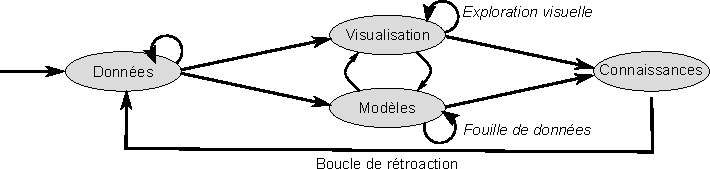
\includegraphics[width=\linewidth]{img/schema_keim.pdf}
	\caption[Itérations entre modèles et visualisations pour enrichir les connaissances.]{Itérations entre modèles et visualisations pour enrichir les connaissances, traduit d'après \textcite[fig.~1, p.~156]{keim_visual_2008}.}
	\label{fig:schema-va}
\end{figure}


\subsection{Comment passer de l'exploration à la validation ? Quelques perspectives \label{subsec:perspectives-validation}}

Dans le \cref{chap:chap3}, on définissait et décrivait les différents enjeux et méthodes de l'évaluation d'un modèle.
Notre approche, sur laquelle les paragraphes précédents constituent quelques retours, est profondément ancrée dans une approche exploratoire et graphique, dénommée \og évaluation visuelle\fg{}.
Au vu des très nombreuses étapes d'évaluation recommandées (cf. \cref{fig:schema_kluegl,fig:schema_ngo} du \cref{chap:chap3}), la question d'une évaluation plus systématique des modèles se pose.
On notait ainsi dans le \cref{chap:chap5} (\cref{subsec:resultats}) que l'évaluation et le calibrage de \simfeodal{} était globalement satisfaisant, mais difficile à prolonger devant l'incomplétude des données empiriques.
Dans les paragraphes suivants, je propose quelques pistes pour améliorer les connaissances sur le modèle, et notamment sur ses qualités en termes de robustesse et de généricité.

\paragraph{Validation interne : quelques pistes pour une exploration plus systématique.}
Une première piste, plusieurs fois évoquée auparavant, est celle des méthodes d'exploration de modèle plus automatisées et systématiques.
Ces méthodes, relatives à la validation interne (voir \cref{chap:chap3}, \cref{enc:lexique-eval-amblard}), permettent d'obtenir une compréhension à la fois plus globale et plus fine du modèle.
Dans la description de l'analyse de sensibilité de \simfeodal{} (\cref{sec:ana-sensib}), je précisais que nous nous étions restreint à une analyse de type \og \textit{one factor at a time}\fg{}, sans faire co-varier les valeurs des paramètres.
Dans le cadre d'un modèle véritablement complexe et doté de très nombreux paramètres qui conditionnent des mécanismes dont l'interaction est importante\footnote{
	Voir par exemple les paramètres agissant de manière contre-intuitive, \cref{subsec:depasser-calibrage}.
}, il est évident que modifier chaque paramètre indépendamment des autres ne permet de rendre compte que d'une faible part de la variabilité que ces derniers peuvent avoir sur les sorties du modèle.
Au contraire, une analyse de sensibilité croisée, testant automatiquement différentes combinaisons de paramètres, permettrait de connaître de manière plus approfondie la gamme de réactions du modèle à des changements de paramètres.
Bien que conceptuellement séduisante, une telle démarche présente des difficultés qui en rendent l'application peu aisée.

Le principal défaut des méthodes croisées tient aux risques d'explosion combinatoire, risques d'autant plus élevés que le modèle est doté de très nombreux paramètres.
Plutôt que de mener des analyses sur le plan complet, des méthodes ont été mises au point pour explorer l'espace des sorties d'un modèle.
Celles-ci permettent, en suivant des heuristiques, de déterminer des sous-ensembles de valeurs à tester, que ce soit en suivant des logiques d'algorithmes génétiques \autocite{schmitt_half_2015,rey-coyrehourcq_plateforme_2015}, des logiques de recherche d'\textit{optima} locaux \autocite{schmitt_modelisation_2014, reuillon_new_2015} ou encore de recherche de motifs dans les sorties \autocite{cherel_beyond_2015}.


Ces méthodes sont extrêmement prometteuses et utiles car elles permettent d'explorer la vaste étendue des comportements d'un modèle en restreignant fortement le nombre de simulations nécessaires.
Elles requièrent toutefois la définition d'un faible nombre d'indicateurs quantitatifs de sortie sur lesquels les différents algorithmes pourront s'appuyer pour définir les valeurs de paramètres à échantillonner.
De plus, l'exemple de l'exploration de l'espace des paramètres du modèle SimpopLocal \autocite{schmitt_modelisation_2014} avec l'une de ces méthodes, \og Calibration Profile\fg{} \autocite{reuillon_new_2015}, montre que pour ce modèle KISS, doté de seulement 5 paramètres, 100 000 heures de calcul machine ont été nécessaires\footnote{
	Réduites à 15 jours de calcul en utilisant les possibilités de calcul distribué mises à disposition par l'infrastructure de calcul intensif EGI.
}.
Sur un modèle moins parcimonieux, le temps nécessaire serait immense, sans même compter la consommation électrique correspondante.
Pour \simfeodal{}, l'apport de connaissances et le raffinement de l'évaluation justifient-ils un tel coût ?
Il me semble que ces méthodes sont strictement inapplicables en l'état actuel du modèle.
Avec un important travail de réduction du nombre de paramètres, de quantification et de synthèse des indicateurs de sortie, elles pourraient apporter des connaissances intéressantes sur le modèle et aider à le rendre plus générique.
Ce n'est toutefois pas la direction qui a été empruntée collectivement dans l'évolution du modèle jusqu'ici. 

Par ailleurs, vu la complexité des données que ces méthodes peuvent produire, il serait à nouveau utile de mener des phases d'exploration et d'interprétation, notamment visuelles, de leurs résultats.
En effet, quelle que soit la complexité et l'efficacité des méthodes de fouille automatique de données ou de modèles, il semble inévitable d'avoir à en mener des analyses visuelles, ne serait-ce que sous la forme de \textit{face validation}, pour en vérifier ou en comprendre les conclusions.
Une plateforme telle que \simedb{} serait entièrement adaptée à l'exploration visuelle des sorties de telles analyses.

\paragraph{Validation externe : données empiriques et confrontation.}
Une seconde piste concerne cette fois-ci la validation externe, c'est-à-dire l'évaluation du modèle au regard des connaissances empiriques dont on dispose sur la période et la région d'étude.
Cette approche, très classique, correspond à la « \textit{statistical validation} » (\cref{chap:chap3}, \cref{fig:schema_kluegl}) ou « \textit{output validation} » (\cref{chap:chap3}, \cref{fig:schema_ngo}).
Dans le cas de \simfeodal{}, j'avais comme projet au début de ce travail de thèse de mener une confrontation, point par point, entre les nombreuses données archéologiques qui ont été compilées pour la Touraine (\cite{rodier2000systeme}, \cite{zadora-rio_paroisses_2008}, par exemple) et les indicateurs correspondants du modèle.
Très vite, j'ai réalisé qu'il serait vain de vouloir comparer les données issues d'un modèle de simulation descriptif et théorique à des données empiriques lacunaires et d'un ordre de généricité bien moindre.
Ces deux types de données présentent des degrés de précision trop différents pour être véritablement comparables.

Hors de la confrontation directe des sorties du modèle avec les données empiriques correspondantes, deux approches complémentaires (voir la \cref{fig:JIG}) pourraient être intéressantes en perspective d'évaluation du modèle \simfeodal{}.
Ces deux approches partent de données historiques et archéologiques pour concevoir des modèles, statistique dans un cas \autocite{gravier_deux_2018} et graphique dans l'autre \autocite{nahassia_formes_2019}.

\begin{figure}[H]
	\centering
	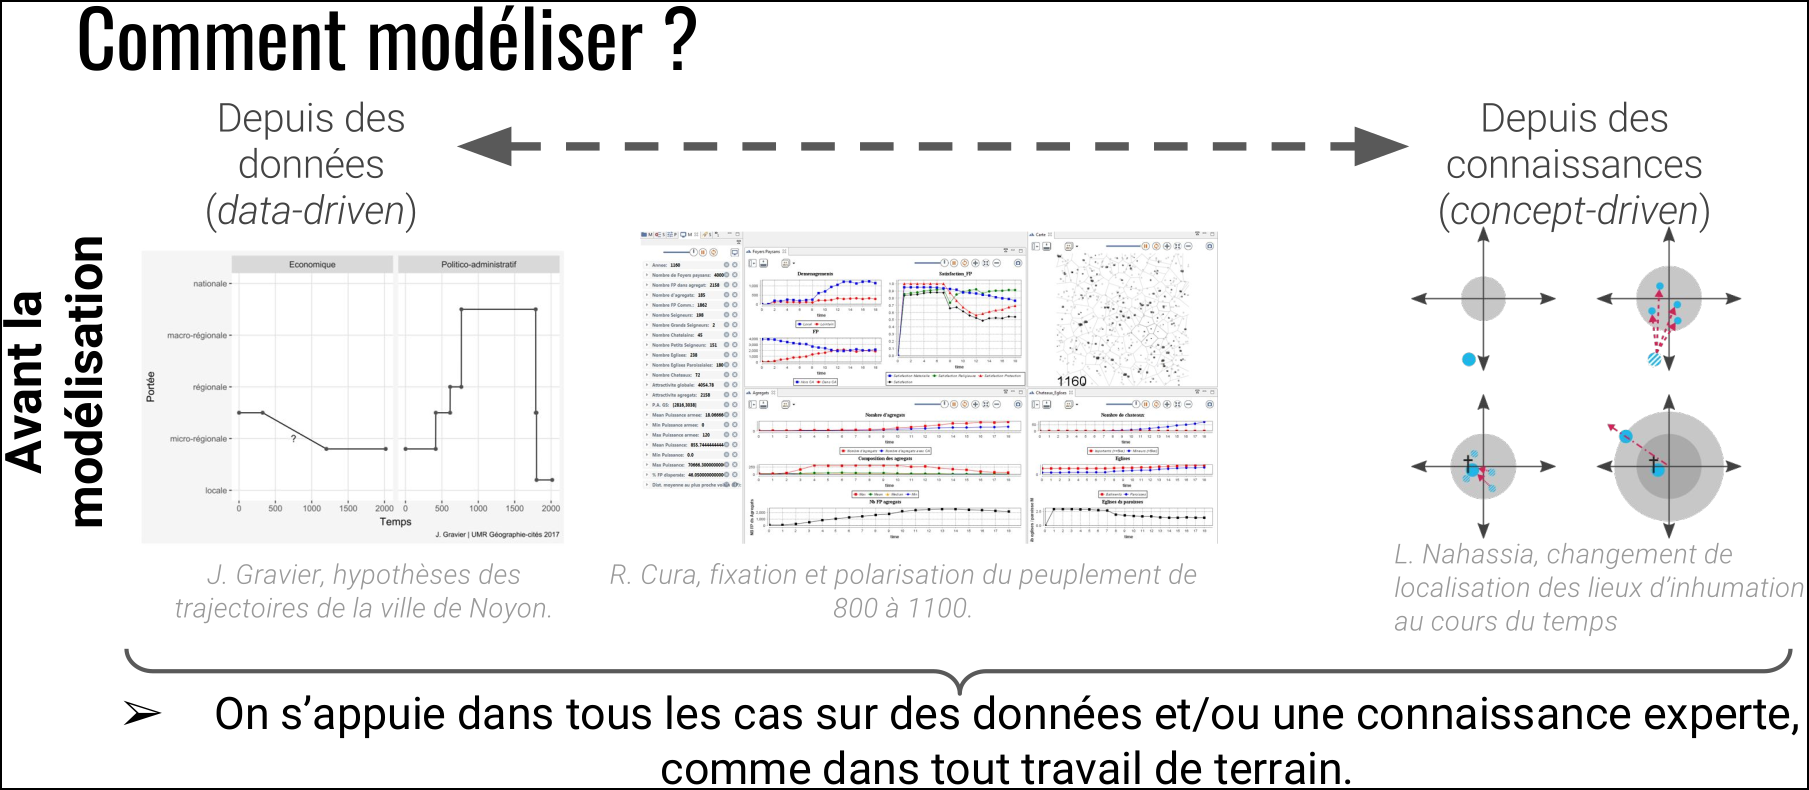
\includegraphics[width=\linewidth]{img/types_modelisation_JIG.png}
	\caption[Trois approches de modélisation différentes de processus sociaux et spatiaux sur le temps long.]{Trois approches de modélisation différentes de processus sociaux et spatiaux sur le temps long \autocite{cura:halshs-02296147}.}
	\label{fig:JIG}
\end{figure}

Dans le cadre de sa thèse dédiée à l'étude d'une ville, Noyon, inscrite dans un système de villes sur la totalité de ses 2000 ans d'existence, \textcite{gravier_deux_2018} prend appui sur la constitution de bases de données harmonisées, d'une résolution très fine et tendant vers l'exhaustivité.
Dans son chapitre 6 \autocite[pp.231--295~]{gravier_deux_2018}, l'auteure mobilise ces données afin d'estimer statistiquement, entre autre, l'importance relative de différents lieux au regard de leurs relations et interactions.
La variété des sources archéologiques et historiques est importante, mais elle est au service d'une seule question thématique.
Ainsi, la diversité thématique des données est assez restreinte.
L'étendue spatiale et temporelle de la zone modélisée est importante, mais comme le questionnement thématique est très circonscrit, la qualité des données permet d'y apporter une réponse robuste.

Pour appliquer cette approche à \simfeodal{}, il s'agirait donc d'aller vers la constitution de bases de données cherchant l'exhaustivité et la précision sur des questionnements plus restreints :
	s'intéresser à des phénomènes très spécifiques, mais en mener une collecte et une analyse très poussée.
On pourrait par exemple chercher des données correspondant à l'un des indicateurs du modèle, comme l'évolution de la distance moyenne à l'église paroissiale la plus proche.
En se gardant d'incorporer ces données lors du calibrage du modèle, on pourrait alors constituer un jeu de données de test, composé de ces données empiriques précises, par lequel éprouver les données de sortie du modèle.

\textcite{nahassia_formes_2019}, quant à elle, étudie dans sa thèse les formes spatiales et temporelles du changement sur la longue durée, à partir du cas de Tours.
La partie 3 \autocite[pp.~239--394]{nahassia_formes_2019} de cette thèse est notamment consacrée à une modélisation graphique des changements de localisation des activités intra-urbaines au cours du temps.
Ces modèles graphiques sont évalués en confrontant les hypothèses théoriques aux riches données dont elle dispose pour la ville de Tours.
Les hypothèses théoriques de l'auteure sont extrêmement générales, et pour les éprouver, elle choisit d'étudier une large diversité de dimensions socio-spatiales tout en réduisant l'amplitude de l'espace étudié à une ville.

En nous inspirant de cette approche, nous pourrions chercher à collecter le maximum d'informations et de données sur une zone à l'étendue restreinte (une paroisse par exemple).
Comme pour l'exemple précédent, on pourrait alors utiliser la correspondance spécifique de l'une des sous-régions modélisées comme critère d'ajustement.
Cette réduction pourrait aussi être temporelle, en ne considérant comme \og crible intermédiaire\fg{}, comme dans la méthode POM \autocite{grimm_pattern-oriented_2005,grimm_pattern-oriented_2012}, que l'accomplissement des faits stylisés choisis sur une partie limitée de la temporalité totale du modèle.

Dans les deux cas, ces possibilités d'évolution de l'évaluation du modèle procèdent de manière assez similaire face à un problème commun.
Il n'est en effet pas possible d'obtenir des éléments empiriques quantifiés sur l'ensemble de la diversité des processus modélisés, sur toute la région et toute la période étudiées.
Une solution serait donc d'ajuster le modèle sur des sous-ensembles témoins de l'une ou plusieurs de ces dimensions (thématique, spatiale, temporelle).
Cette approche est fréquemment utilisée pour les modèles statistiques prédictifs (scénarios démographiques et climatiques entre autre), qui peuvent par exemple avoir pour point de départ temporel une période relativement récente, et où l'on cherche à ce que les \og rétro-prédictions\fg{} correspondent aux données empiriques déjà connues au moment de la création du modèle.


\paragraph{Validation croisée : désancrer le modèle pour en évaluer la généricité.}\label{par:validation-croisee}
Une dernière piste, évoquée dès les prémices de ce travail de thèse, consisterait à mener une évaluation par le biais de \og scénarios régionaux\fg{}.
Dans le chapitre précédent, je présentais une analyse de scénarios thématiques qui nous paraissent intéressants au regard des questionnements des archéologues et historiens de notre groupe de travail.
Ces scénarios sont plausibles et doivent aider aussi bien à tester la robustesse du modèle face à des changements conséquents de valeurs de paramètres qu'à évaluer la réaction des interactions entre mécanismes dans des contextes thématiques légèrement différents (augmentation de la part des foyers paysans dépendants -- serfs et esclaves -, hypothèses de croissance démographique, etc.).

Les scénarios que nous mentionnons ici et qui pourraient participer à l'évaluation du modèle seraient plutôt des scénarios régionaux, c'est-à-dire qu'ils viseraient à adapter les valeurs calibrées du modèle à d'autres contextes spatiaux et temporels.
En effet, \simfeodal{} est un modèle qui se veut générique à l'Europe du Nord-Ouest, mais qui a été calibré sur une région particulière : la Touraine.
En désancrant le modèle, c'est-à-dire en l'adaptant à une autre région dotée de paramètres différents, on pourrait ainsi procéder à une sorte de validation croisée (\textit{cross validation}).
Si le modèle, une fois ses \textit{inputs} et paramètres de contexte adaptés à la description d'une autre région produit des résultats plausibles pour les experts thématiciens de cette autre région, alors on peut considérer que \simfeodal{} réussit à reproduire les faits stylisés recherchés de manière plus robuste qu'initialement.
Par exemple, on sait que les faits stylisés modélisés dans \simfeodal{} sont génériques à l'Europe du Nord-Ouest, mais selon des rythmes et des proportions potentiellement propres à chaque région.
Si l'on prend le cas d'un diocèse montagnard, on pourrait alors diminuer les différents seuils de distance paramétrés selon des connaissances d'experts pour tenir compte du relief plus difficile à franchir, aboutissant à des temps de parcours plus importants.
Aboutirait-on à une concentration des foyers paysans plus lente et moins nette ou, au contraire, est-ce que ce processus serait accéléré et accentué ?
En travaillant avec des spécialistes de l'histoire de ces régions, on pourrait ainsi tester la validité des hypothèses du modèle sur leurs propres terrains d'expertise.


\textit{A posteriori} de ce travail, un séminaire visant à éprouver \simfeodal{} sur d'autres régions, dans lesquelles les historiens trouvent des similarités générales de changement de structure spatiales et sur lesquelles les sources empiriques paraissent suffisantes (Normandie, Champagne, Lorraine, Alsace, Flandre, Poitou, Provence, Quercy, etc.), est d'ailleurs déjà prévu.
Là encore, pour le dialogue interdisciplinaire et inter-régional, l'utilisation, grâce à \simedb{}, de représentations graphiques interactives comme interface entre les chercheurs présentera sans doute les avantages discutés dans ce travail de thèse.

\subsection{Conclusion : Pour un recours systématique à la visualisation dans l'analyse de modèles}

Dans cette partie, je suis revenu sur les bénéfices que l'analyse exploratoire visuelle a pu apporter dans le cadre de notre expérience interdisciplinaire de conception et de développement de modèle, dont \simfeodal{} est le résultat.
Plus largement, ce retour d'expérience conforte l'idée que la modélisation pourrait profiter d'un recours plus systématique à l'analyse visuelle des données produites.
Cela me semble résonner d'autant plus dans le cas des modèles spatiaux, tant la pratique de la représentation graphique est ancrée dans la culture disciplinaire des géographes.
On ne peut toutefois, parallèlement, que constater la faiblesse de la production (carto)graphique dans le domaine de la modélisation \autocite[Introduction]{cura_visualisation_2020}, alors même que les plateformes de simulation multi-agents rivalisent de possibilités en ce sens.

Nous l'avons vu, la visualisation peut aider le modélisateur et les spécialistes thématiciens qui l'entourent tout au long du cycle de développement d'un modèle :
	dès sa conception, en participant à la co-construction et au travail collaboratif (la visualisation comme interface interdisciplinaire, comme formalisme d'explicitation des composantes et sorties d'un modèle, etc.) ; mais aussi, une fois le modèle implémenté, comme outil d'évaluation et support à une potentielle validation des modèles (validation interne, méthodes d'exploration automatiques et validation croisée).
En cela les modélisateurs auraient, il nous semble, tout intérêt à s'emparer de la question de la visualisation.

Pour que ces apports soient complets et utiles à tous, le transfert disciplinaire ne peut être à sens unique :
	là où les géographes peuvent bénéficier des recherches en visualisation de données, ces dernières gagneraient aussi à pourvoir aux problématiques propres aux données issues des modèles de simulation géographiques qui ont été esquissées ici (\cref{subsec:genericite-donnees-simul}).
Pour reprendre \textcite[76]{banos_pour_2013}, \og il ne suffit pas de mettre en contact des disciplines pour que l'interdisciplinarité émerge.
La pluridisciplinarité s'en contente facilement, mais l'interdisciplinarité implique des interactions entre disciplines et par conséquent une nécessaire acculturation [...].
Donner les moyens aux géographes et, au delà, aux chercheurs en sciences humaines et sociales, de devenir plus autonomes dans leur démarche de [visualisation\footnote{
	\og Modélisation\fg{} dans le texte original.
}] va [aussi] dans ce sens\fg{}.


\clearpage
\let\orisectionmark\sectionmark
\renewcommand\sectionmark[1]{}%
\section{Retours sur la co-construction d'un modèle de simulation descriptif\label{sec:retour-coconstruction}}
\orisectionmark{Retours sur la co-construction d'un modèle de simulation descriptif}
\let\sectionmark\orisectionmark

Tout au long de ce travail de thèse, nous avons choisi de tenir un positionnement réellement collectif et collaboratif.
Nous souhaitions, comme annoncé dans le \cref{chap:chap1}, co-construire un modèle plutôt que construire un modèle \og pour\fg{} des collègues historiens et archéologues.
Le travail de modélisation qui a abouti à \simfeodal{} a été initié au sein du projet ANR TransMonDyn, préalablement au début formel de ce travail de thèse.
Ce travail de modélisation n'est d'ailleurs pas achevé :
	son cadre dépasse celui de la thèse, et des projets en cours, voire à l'état d'initialisation, sont encore prévus pour faire vivre le modèle \simfeodal{} et la démarche qui en a animé la construction, l'évaluation et l'utilisation.
Ce manuscrit est l'occasion de réaliser un point d'étape dans ce processus de modélisation qui s'inscrit résolument sur la longue durée, relativement à l'échelle de la recherche.
Le retour d'expérience que constitue ce travail de thèse s'est relativement affranchi d'une présentation chronologique des différentes étapes de développement du modèle.
Pour autant, il me semble nécessaire ici de dresser un bilan réflexif revenant sur les conditions souhaitées de construction du modèle \simfeodal{} au regard de celles qui se sont concrètement réalisées.

Dans le \cref{chap:chap1} (\cref{subsec:co-construction}), j'ai présenté l'approche ComMod (Modélisation d'accompagnement) en identifiant les différences avec la démarche que nous souhaitions mener dans cette expérience de modélisation collective.
Les points de divergence présumés étaient, d'une part, la volonté forte d'aller jusqu'au modèle implémenté dans notre projet, ce qui n'est pas systématiquement fait dans l'approche ComMod et, d'autre part, la séparation entre \og animateurs\fg{} et \og participants\fg{} dans l'approche ComMod, qui correspond à une distinction des rôles que nous souhaitions effacer dans un processus de co-construction.
Dans cette partie, je reviens sur ces deux points de divergence présumés pour discuter de leur validité réelle, \og \textit{a posteriori}\fg{} de l'expérience de co-construction de modèle.
Enfin, dans un retour sur les deux premiers chapitres, qui présentaient \simfeodal{} comme un modèle exploratoire et descriptif et justifiaient ce choix, je discute la position effective du modèle.
Ce sera l'occasion de revenir sur l'évolution de cette position au cours des différentes versions du modèle et donc d'appréhender quelle a été la trajectoire de \simfeodal{} jusqu'ici.

\subsection{Un retour d'expérience critique sur l'usage de modèles de simulation descriptifs : les limites de l'implémentation}

L'expérience constituée par ces nombreuses années de travail sur le modèle \simfeodal{} a été enrichissante sur tous les plans, mais ce retour d'expérience est aussi l'occasion de pointer certains obstacles rencontrés, parfois non surmontés, quant à l'utilisation effective du modèle de simulation.
Dès le départ, nous avions fixé un rôle exploratoire au modèle, en en faisant avant tout un support à la pensée.
Nous avions toutefois l'ambition de pouvoir tester les hypothèses thématiques, non pas pour les (in)valider, mais pour être en mesure de vérifier s'il était possible que ces hypothèses puissent être nécessaires et suffisantes pour reproduire les processus empiriques étudiés.

\paragraph{Quel usage pour un modèle de simulation descriptif et exploratoire ?}

Aujourd'hui, il me semble que cette ambition n'est pas entièrement -- ou pas encore -- satisfaite.
Un premier problème, commun à tous les types de modèle, est celui de l'équifinalité -- bien conceptualisé notamment dans le domaine de la simulation en archéologie \autocite{premo_equifinality_2010}.
Comme indiqué dans \textcite[415]{reycoyrehourcq:hal-01677950}, l'équifinalité
	\og désigne de façon générale la possibilité d'obtenir, pour un système ouvert, un état final identique en suivant des trajectoires et des conditions initiales variées.
	Cela signifie dans le cas d'un modèle de simulation que des jeux d'hypothèses ou de paramètres différents peuvent mener à des résultats identiques\fg{}.
Quel que soit le mode et la qualité de \og validation\fg{} d'un modèle, celui-ci ne constituera jamais plus et au mieux qu'un \og candidat à l'explication\fg{}.

Dans le cas des modèles descriptifs ou exploratoires, fondés sur de très nombreux mécanismes, il me semble que ce dernier constat est renforcé.
En effet, dans un modèle, chaque mécanisme peut être conçu, puis implémenté de plusieurs manières.
En multipliant les mécanismes, on augmente d'autant le nombre de solutions alternatives possibles, et on augmente exponentiellement le nombre de combinaisons potentielles résultant de ces alternatives possibles.
Dans un modèle statistique, à mesure que l'on ajoute des variables, on augmente presque mécaniquement l'ajustement global du modèle aux données étudiées.
Même sans ajouter de variables explicatives, on peut aussi renforcer l'ajustement d'un modèle quelconque en en complexifiant la formulation.
Par exemple, pour une même série de point que l'on chercherait à décrire par une régression polynomiale, plus le degré de ce polynôme augmente, plus l'ajustement est amélioré lui aussi.
Est-ce pour autant, dans le cas de points corrélés plutôt linéairement (voir \cref{fig:regression-polynomiale}), que la variable explicative est plus valide, sur un plan thématique, qu'avec une régression polynomiale de degré 1, c'est-à-dire une régression linéaire ?
 
\begin{figure}[H]
	\centering
	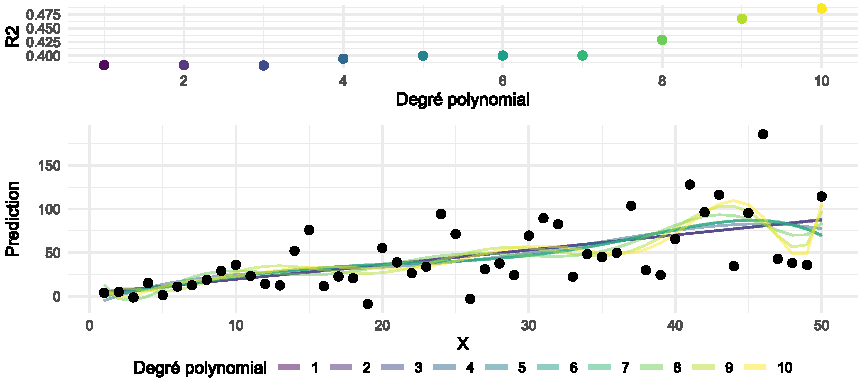
\includegraphics[width=\linewidth]{img/regression_polynomiale.pdf}
	\caption{Un exemple de sur-ajustement d'une série de points avec l'augmentation du degré d'une suite de régressions polynomiales.}
	\label{fig:regression-polynomiale}
\end{figure} 
 
Dans un modèle très stylisé où seuls quelques mécanismes sont présents, on est capable d'affirmer que la conjonction de ces mécanismes est un candidat potentiel à l'explication, voire d'éliminer d'autres candidats potentiels à l'explication, par exemple, avec le principe de parcimonie.
Dans un modèle plus descriptif, l'accumulation de choix de mécanismes et de leurs interactions, difficiles à maîtriser, me semble rendre plus difficile cette affirmation.
Dans l'exemple de \simfeodal{}, on cherchait à pouvoir affirmer que la polarisation et la hiérarchie du système de peuplement pouvaient être expliquées par des dynamiques liées à l'émiettement des pouvoirs, l'augmentation de la violence et l'augmentation de l'encadrement religieux.
Dans l'état actuel du modèle, le risque est que ce soit la somme des choix spécifiques liés aux modes d'interactions entre les mécanismes qui aboutissent en un modèle dont les résultats sont satisfaisants, tandis que les mêmes mécanismes, agencés différemment, aboutiraient peut-être à des résultats très différents.

\paragraph{Validité interne d'un modèle complexe.}
Ce constat est accentué par la nature complexe (en termes de complexité algorithmique) de l'implémentation informatique, qui en rend nécessairement l'évaluation interne plus difficile.
Avec un modèle composé de plusieurs dizaines de mécanismes et donc de quelques milliers de lignes de code comme \simfeodal{}, le risque d'erreur -- méthodologique ou technique -- est infiniment plus important que sur un modèle-jouet composé de quelques mécanismes et de quelques dizaines de lignes de code.
Lors du paramétrage de \simfeodal{}, de très nombreuses erreurs ont été détectées et corrigées :
	parfois le code ne correspondait pas au mécanisme tel qu'il avait été défini, parfois le choix de telle ou telle fonction informatique ne retournait pas le résultat décrit dans la documentation de la plateforme de simulation (GAMA), parfois un mécanisme du modèle était court-circuité par un autre (informatiquement ou conceptuellement), etc.
Il est habituel, et presque attendu, qu'un programme informatique contienne des erreurs ou \textit{bugs}, mais en complexifiant ce programme, on augmente fortement ce risque d'erreur.


Ces erreurs sont le plus souvent de la responsabilité de ceux qui implémentent le modèle, mais parfois, elles dépendent aussi d'éléments difficiles à contrôler, telle que la présence d'erreurs au sein même des outils utilisés pour mener la modélisation.
C'est un risque inhérent à l'utilisation de plateformes de modélisation \og de recherche\fg{} :
	les développeurs de ces outils sont tout autant susceptibles de commettre des erreurs d'implémentation que les modélisateurs.
Ils en commettront sans doute proportionnellement moins qu'un non-informaticien, mais la complexité du code n'est pas du même ordre de grandeur non plus.
La plateforme de simulation GAMA, par exemple, repose sur plus de 500 000 lignes de code.
Parmi celles-ci, la probabilité qu'il n'y ait aucune erreur est quasi-nulle, en dépit des très nombreux et réguliers \textit{commits} qui viennent, justement, corriger ces \textit{bugs}.
Une bonne partie de ces \textit{bugs} sont en fait peu dommageables dans le cas de \simfeodal{}, parce qu'ils portent sur des fonctions non utilisées, ou sur des conjonctions de cas non rencontrés dans le modèle.
Cependant, une erreur importante concernant l'ordonnancement des agents a été détectée et corrigée sur la plateforme GAMA en mai 2016, dont la version était alors jugée stable (version 1.7).
Cette erreur, survenue entre les versions 3 et 4 de \simfeodal{} (voir \cref{chap:chap3}, \cref{tab:historique-versions-simfeodal}) a eu des conséquences majeures sur les résultats du modèle, et une large partie des expériences réalisées précédemment à la correction de ce bug a du être ré-exécutée pour en vérifier les sorties une fois le bug corrigé.

Dans une perspective thématique, où l'on cherche à tester des hypothèses, un modèle descriptif est alors moins robuste qu'un modèle KISS.
C'est autant vrai pour l'aspect conceptuel -- la multiplicité des interactions entre mécanismes étant difficilement contrôlable -- que pour l'aspect informatique où les risques d'erreurs sont multipliés.
Lors du passage du modèle conceptuel au modèle implémenté, il y a de fortes chances que des erreurs des modélisateurs viennent invalider les résultats thématiques proposés grâce au modèle.
Même dans un modèle parfaitement implémenté, l'équifinalité conceptuelle, les choix techniques d'implémentation, ou encore les potentielles erreurs des plateformes logicielles utilisées peuvent restreindre la qualité démonstrative du modèle :
	ce ne sont pas les hypothèses conceptuelles, seules, intégrées dans le modèle qui pourront constituer des candidats à l'explication thématique mais les hypothèses telles qu'elles ont été construites et formalisées dans le modèle implémenté.


\paragraph{De l'importance de l'implémentation.}
Dans le cadre d'une démarche collective de modélisation, ces quelques limites, inhérentes au choix d'une modélisation informatique de type descriptive, ne sont toutefois pas véritablement gênantes au vu des nombreux atouts de ce type de démarche -- introduits dans le \cref{chap:chap1}.
L'implémentation informatique du modèle a nettement renforcé le besoin d'explicitation des hypothèses introduites.
Plus le formalisme employé est précis et non ambigu (ce qui est le cas des formalismes informatiques et non des modèles \og rhétoriques\fg{} ou \og graphiques\fg{} évoqués dans l'\cref{chap:intro}), plus leur utilisation force à préciser et à expliciter la conceptualisation du modèle.
En allant jusqu'à l'implémentation informatique, nous avons collectivement été amenés à trancher des centaines de choix, à expliciter à de multiples reprises le contenu de chacun des nombreux mécanismes, et donc à élaborer, ensemble, une compréhension partagée de ce modèle pour la totalité des domaines qui le caractérisent.
De plus, un modèle de simulation descriptif est un outil dont la multiplicité des composantes (mécanismes, agents, interactions entre mécanismes, etc.) favorise l'exécution d'incessantes modifications, que ce soient des corrections ou des améliorations.
La correction de chaque erreur conceptuelle est l'occasion de re-vérifier (au sens d'une validation interne) la cohérence d'ensemble des composantes du modèle.
Chaque bug informatique corrigé dans une fonction du modèle implémenté permet de vérifier le bon fonctionnement et la robustesse des autres fonctions.
Les rapports d'erreur, au niveau de la plateforme de simulation, donnent l'occasion d'améliorer le code du modèle en le rendant plus robuste.
Chacune de ces erreurs, mais aussi chacune des améliorations localisées qui sont appliquées au modèle, permettent ainsi de revoir la cohérence du modèle dans sa globalité.
Toutes ces interventions sur le modèle, conceptuelles autant qu'informatiques, contribuent à renforcer progressivement la confiance que l'on peut lui accorder thématiquement. Un modèle \og entretenu régulièrement\fg{} comme \simfeodal{} constitue ainsi un support à la discussion dont la \og durée de vie\fg{} me paraît supérieure à celle d'un modèle plus simple, parce que les possibilités de reprises et de raffinement sont nombreuses.

\subsection{Quelle part effective du collectif dans la conception et l'implémentation du modèle ?}

Tout au long du manuscrit de cette thèse, j'ai insisté sur la dimension collective de co-construction qui a permis d'aboutir au modèle \simfeodal{}.
On pourrait objecter, au regard des \textit{commits} du modèle, que seules deux personnes ont effectivement apporté des modifications dans le dépôt logiciel.
En regardant plus en détail l'historique de ce dépôt, on pourrait même constater que Cécile \textsc{Tannier}, l'autre contributrice du dépôt, n'est intervenue \og que\fg{} dans de nombreuses modifications de la documentation du modèle.
Le code-source de \simfeodal{} n'a donc été implémenté, en tant que tel, que par moi.

Cela signifie-t-il pour autant que la volonté de co-construction globale, du modèle conceptuel jusqu'au modèle implémenté, n'a finalement pas été entièrement effective ?
Avant de répondre à cette question, je crois important d'expliquer la décision de cette implémentation mono-participante, qui pourrait largement accréditer la distinction entre \og participant\fg{} et \og animateur\fg{} (ou \og implémenteur\fg{}, voir \cref{chap:chap1}, \cref{subsec:co-construction}).

\paragraph{Compétences spécifiques nécessaires pour l'implémentation d'un modèle de simulation.}
Le développement informatique d'un modèle de simulation demande des compétences particulières.
En premier lieu, des compétences méthodologiques, relatives à la capacité à transcrire sous forme algorithmique les mécanismes et interactions exprimés dans un modèle conceptuel.
Ces compétences sont l'une des caractéristiques attendues d'un \og modélisateur\fg{}, et assez répandues dans les sous-domaines quantitatifs des sciences humaines et sociales.
En second lieu, le développement d'un modèle de simulation requiert des compétences techniques assez spécifiques et avancées.
Les algorithmes et fonctions doivent en effet nécessairement être \og implémentés\fg{} informatiquement, c'est-à-dire écrits, \og développés\fg{}, dans un langage de programmation, qui doit donc être maîtrisé par le modélisateur.
Dans le monde de la simulation à base d'agents, les différentes plateformes disponibles mobilisent de nombreux langages de programmation.
Dans une étude globale portant sur 24 plateformes, \textcite{kravari_survey_2015} montrent ainsi que l'on retrouve 14 langages de programmation différents \autocite[table 7, \S 4.3]{kravari_survey_2015}.
Certains sont très génériques (Java, C/C++, Python, etc.), tandis que d'autres ont été créés spécifiquement pour la plateforme de simulation correspondante (langage Logo pour NetLogo, langage GAML pour GAMA, etc.).

Un modélisateur formé dans l'un de ces langages de programmation, et en particulier ceux spécifiques à la simulation multi-agents, aura indéniablement plus de facilités à en apprendre un autre.
Cela demande tout de même un apprentissage conséquent, le plus souvent réalisé par auto-formation.
\simfeodal{} a été développé sur la plateforme GAMA, en langage GAML, qu'aucun des membres du projet ne maîtrisait réellement.
L'acquisition par tous les participants de la connaissance de ce langage aurait donc demandé un temps important d'apprentissage, pas nécessairement utile au regard de l'objectif du projet.

\paragraph{Des compétences à entretenir et à développer.}
En plus du coût temporel de formation initiale, l'utilisation d'une plateforme de simulation \og de recherche\fg{} requiert aussi une formation continue puisque la plateforme sur laquelle le modèle est bâti évolue.
Au cours du développement de \simfeodal{}, trois versions \og majeures\fg{} successives de GAMA ont par exemple été utilisées (1.6, puis 1.7 et finalement 1.8).
Chacune de ces versions apporte des améliorations qui permettent notamment de gagner en performance, en stabilité, ou de disposer de nouvelles fonctions qui permettent une meilleure expressivité du code.
On peut faire le choix de construire le modèle à partir d'une seule et unique version, quand bien même celle-ci serait obsolète au bout d'un moment, mais cela revient à négliger toutes ces améliorations.
De plus, lorsque les nouvelles versions de la plateforme viennent corriger des erreurs latentes, ce qui est le cas de GAMA, il est essentiel de mettre à jour le logiciel.
L'implémentation informatique d'un modèle dans ces conditions requiert donc un travail incessant de mise à jour, de correction et d'optimisation du code-source du modèle.
Cela implique un coût temporel important de formation, de veille technologique, mais aussi de retours d'expériences aux développeurs de la plateforme, de rapports de \textit{bug} (\textit{issues}) et de demande d'améliorations (\textit{enhancements}), sans même aborder le temps nécessaire à l'implémentation effective.
Même si, dans notre groupe de travail, Cécile \textsc{Tannier} s'est formée en GAMA pendant le développement de \simfeodal{} ou que Samuel \textsc{Leturcq} a suivi des formations MAPS pour apprendre le Logo, leur participation effective à l'écriture du code de \simfeodal{} aurait demandé un temps important.
Temps d'autant plus important si l'on considère que le développement collectif (par opposition au développement individuel) requiert encore d'autres compétences :
	maîtrise d'outils collaboratifs (versionnement collaboratif par exemple), bonne connaissance du langage pour comprendre le code développé par les autres, et plus encore pour en comprendre l'intention et la logique d'organisation\ldots
Ce dernier point est d'autant plus prégnant que le modèle est déjà, en lui-même, complexe :
	le temps nécessaire à la familiarisation à son code augmente.

\paragraph{Une construction effectivement collective.}

Pour autant, le développement collectif apporte un avantage indéniable en matière d'évaluation interne du modèle développé :
	en multipliant les points de vue sur le code, on multiplie d'autant les probabilités de débusquer les erreurs d'implémentation.
Ces points de vue peuvent émaner de différentes personnes, mais aussi être suscités de la part d'un unique individu.
C'est par exemple au fondement de la méthode de validation interne du \og \textit{rubber duck}\fg{} \autocite{noauthor_methode_2019}, où l'on explique à un objet (un \og canard en plastique\fg{} classiquement) son code en le commentant ligne par ligne.
L'objectif de cette oralisation du code est de le présenter d'une autre manière, et par conséquent d'y repérer des erreurs qui auraient échappé à sa \og lecture\fg{}.

Dans le cas de \simfeodal{}, et cela constitue un début de réponse à l'interrogation sur l'effectivité de la co-construction du modèle, nous avons bénéficié d'oreilles bien plus attentives qu'un canard en plastique auprès des participants au projet.
Toutes les lignes de code correspondant aux mécanismes du modèle ont systématiquement été oralisées, explicitées et discutées, au moins par les deux \og modélisateurs\fg{} du groupe.
Au-delà de cette vérification, toute la conception algorithmique de ces mécanismes en elle-même a été réalisée collectivement, impliquant chacun en fonction de ses aptitudes, c'est-à-dire surtout les modélisateurs, mais avec une participation sensible des thématiciens, notamment en termes de validation ou d'arbitrage.
La manière de concevoir et d'implémenter les mécanismes de \simfeodal{} résulte de décisions unanimes vis-à-vis de la meilleure manière de rendre compte des intuitions collectives, incluant autant les modélisateurs que les thématiciens. 

Face à un modèle informatique, exprimé dans un formalisme qu'ils ne maîtrisent pas, les chercheurs dotés d'expertise thématique procurent une aide majeure en cas de doute entre des mécanismes alternatifs possibles par exemple.
Ce sont en effet le plus souvent eux qui ont tranché à partir de leur connaissance experte des phénomènes.
Par ailleurs, comme dans la technique du \textit{rubber duck}, les mécanismes leur ont tous été décrits de manière précise, c'est-à-dire en explicitant leur contenu à partir du code-source, que ce soit verbalement ou à l'aide de représentation graphiques (schémas, diagrammes d'activité, etc.).
Ces pratiques ont contribué à la validation interne du modèle (explicitation et multiplication des points de vue) autant qu'à sa validation externe (par le jugement des thématiciens sur les détails d'implémentation du modèle).
Notons enfin que l'influence des membres du projet qui n'ont pas participé aux dernières années de la modélisation de \simfeodal{}, l'archéologue Élisabeth \textsc{Lorans} et le \og modélisateur-archéologue\fg{} Xavier \textsc{Rodier}, a été importante et est toujours visible dans certains choix d'implémentation de la version actuelle de \simfeodal{} (définition conceptuelle et algorithmique des agrégats notamment).


\paragraph{Un processus de co-construction inscrit dans la durée.}
Au regard de cette expérience, il me semble que la volonté de co-construire le modèle en impliquant chaque membre du projet lors de chacune de ses étapes a été relativement respectée.
Comme expliqué dans le \cref{chap:chap1}, les \og thématiciens\fg{} ne sont pas devenus pour autant des experts en implémentation de modèle de simulation, et les \og modélisateurs\fg{} n'ont pas acquis l'ensemble des compétences disciplinaires de leurs collègues.
La recherche d'une posture -- idéale -- de \og modélicien\fg{} (\textsc{Banos}, in \cite[484]{ouriachi_lelaboration_2017}) n'est pas entièrement aboutie, mais le temps long de ce processus de modélisation collective a cependant permis à tous de participer à chacune des phases du projet.
Les thématiciens, qui ne sont pas les simples \og participants\fg{} comme dans l'approche ComMod, ont ainsi fortement contribué à la construction en tant que telle du modèle implémenté, fournissant également de nombreux retours sur ce dernier.
Il me semble que c'est justement ce temps long qui a permis la construction collective de \simfeodal{}, en laissant à chacun le temps de s'acclimater aux positions et demandes des autres.

L'implication collective sur le temps long, relativement au temps court et parfois urgent de certaines expériences de modélisation dans un contexte de recherche-action, a été facilitée par l'organisation très horizontale qui a toujours caractérisé notre groupe de travail, horizontalité rendue possible par l'usage avant tout exploratoire et heuristique du modèle.
Il n'y avait ainsi ni sensibilisation à un aléa, ni besoin de conciliation entre des acteurs, mais simplement une curiosité scientifique sur l'importance qu'un modèle de simulation pourrait constituer comme support à la pensée d'un ensemble de processus sociaux inscrits dans l'espace et dans la durée.
En cela, l'expérience \simfeodal{} a effectivement été -- et continuera sans doute de l'être après le rendu de ce manuscrit -- mue par une démarche de co-construction profondément exploratoire et abductive, les résultats et discussions intermédiaires guidant la suite de l'évolution du modèle.

\subsection{La trajectoire du modèle SimFeodal}

La démarche exploratoire qui a guidé la co-construction de \simfeodal{} a aussi entraîné une forte évolution du modèle.
Dans le \cref{chap:chap3} (\cref{tab:historique-versions-simfeodal}), j'ai déjà présenté l'historique des versions du modèle, de même qu'une analyse quantitative rétrospective de son mode de progression méthodologique.
Au-delà du modèle implémenté, il me semble intéressant de revenir sur la matérialisation de cette démarche exploratoire, que l'on peut retracer au travers de la matérialisation de l'évolution du modèle conceptuel, c'est-à-dire de sa trajectoire.

\paragraph{Référentiel de la trajectoire.}
Pour décrire une trajectoire, il faut définir deux éléments : un référentiel et un point d'origine.
Comme référentiel, on peut utiliser le cadre du \og fer à cheval\fg{}, développé par \textcite{banos2012vers} et explicité par les mêmes auteurs l'année suivante \autocite{banos2013modeliser}.
Ce cadre vise à la représentation des modèles et de leurs trajectoires dans un référentiel constitué de deux axes.
L'axe des abscisses est un gradient du \og niveau de simplification du modèle\fg{}, s'étendant des modèles jugés \og KISS\fg{}, c'est-à-dire très simplifiés, jusqu'aux modèles \og KIDS\fg{}, peu simplifiés \autocite[840-841]{banos2013modeliser}.
L'axe des ordonnées correspond au \og niveau d'abstraction du phénomène empirique que l'on cherche à modéliser\fg{}, qui peut être résumé en \og phénomène particulier ou fait stylisé\fg{} \autocite[839-840]{banos2013modeliser}.
Pour les auteurs, l'intersection de ces deux axes de description permet de positionner et de différencier les modèles de systèmes spatiaux.

Pour illustrer l'usage de ce référentiel, le travail de \og modélographie\fg{} de \textcite{schmitt_modelographie_2013} constitue un bon exemple.
Dans cet article, les autrices décrivent et comparent six modèles multi-agents géographiques qui simulent des interactions entre des sociétés et leur environnement spatial.
Chacun des modèles est présenté selon une grille de description commune\footnote{
	Les autrices n'utilisent pas le formalisme ODD \autocite[\S 5-6]{schmitt_modelographie_2013} et proposent une grille personnelle : \og contexte de recherche\fg{}, \og enjeux de modélisation\fg{}, \og dynamiques simulées\fg{} et \og sorties de simulations et résultats\fg{}.
}, et l'un des résultats est notamment constitué par une comparaison graphique des positions des modèles dans le référentiel du \og fer à cheval\fg{} (\cref{fig:modelographie}).


\begin{figure}[H]
	\centering
	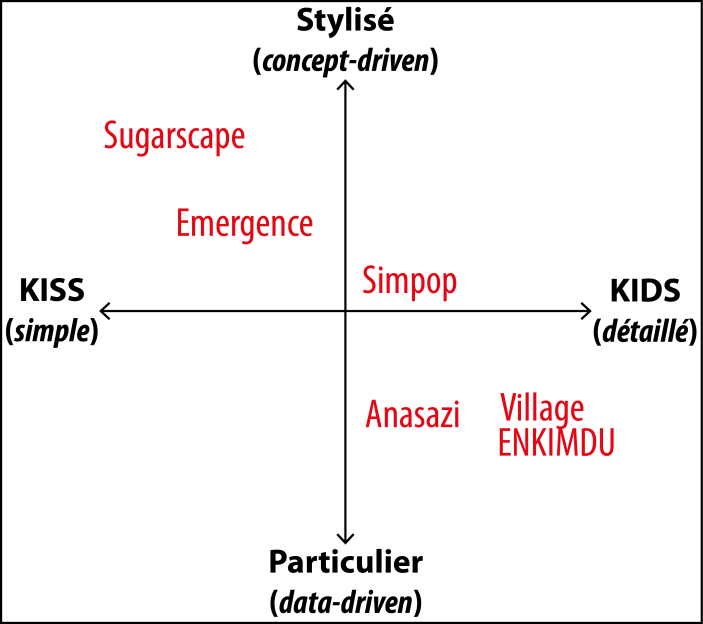
\includegraphics[width=.725\linewidth]{img/modelographie_fer-a-cheval.png}
	\caption[Une \og classification des approches de modélisation\fg{} de modèles géographiques.]{Une \og classification des approches de modélisation\fg{} de modèles géographiques, tirée de la \og modélographie\fg{} \textcite[Figure 1]{schmitt_modelographie_2013}.}
	\label{fig:modelographie}
\end{figure}


\paragraph{Origine de la trajectoire.}
La définition du point d'origine d'un modèle dans ce référentiel est plus difficile car éminemment subjective.
Selon le point de vue de celui qui positionne le modèle, qu'il participe ou non à sa construction, la position peut ainsi varier.
On peut le montrer en s'appuyant sur un exercice qui avait réalisé à la fin du projet TransMonDyn, où un groupe de travail avait cherché à mener une \og TransModélographie\fg{}, c'est-à-dire une comparaison systématique des différents modèles construits au sein du projet.
Pour mener ce travail, nous avions commencé par présenter notre démarche aux différents participants du projet, en proposant notamment une classification \og naïve\fg{} des modèles de chacun (\cref{fig:transmodelographie}).

\begin{figure}[H]
	\centering
	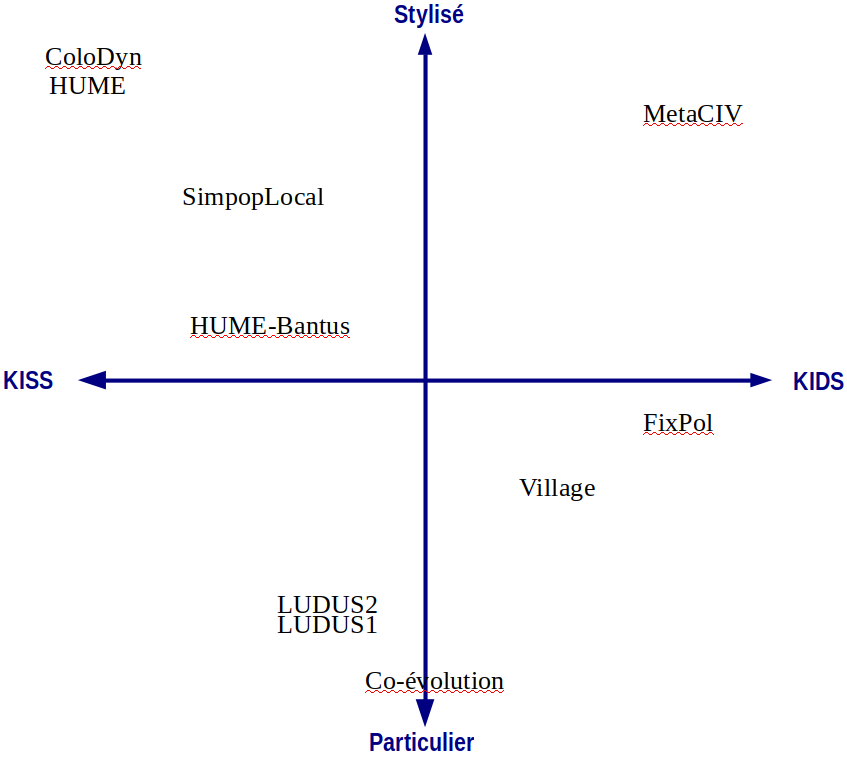
\includegraphics[width=\linewidth]{img/transmodelographie.png}
	\caption[Une proposition de \og TransModélographie\fg{}.]{Une proposition de \og TransModélographie\fg{}.\\
	Figure issue d'une communication à un séminaire interne du projet TransMonDyn à Tours, Octobre 2014, par Robin \textsc{Cura}, Hélène \textsc{Mathian} et Clara \textsc{Schmitt}.\\
	\textit{N.B. : Le modèle \og FixPol\fg{} (fixation et polarisation) est un ancien nom de \simfeodal{}.}}
	\label{fig:transmodelographie}
\end{figure}
%TODO : Faire référence au tableau des transitions (\cref{chap:chap1}, \cref{tab:transitions-tmd})) en disant à quelle transition chaque modèle correspond

À la suite de cette présentation, nous avions demandé aux participants de remplir un questionnaire visant à décrire selon leur point de vue la position du modèle auquel ils participaient.
Faute de temps, ce projet n'a pas pu être mené à son terme, mais suite au dépouillement des premières réponses, nous avions noté la forte hétérogénéité des descriptions d'un même modèle, selon le rôle de l'intervenant (thématicien, modélisateur), mais aussi une hétérogénéité parmi les différents tenants d'un même rôle au sein d'un même modèle.
Les modèles ne changeaient pas réellement de cadran, mais en leur sein, la position déclarée par chacun variait fortement.

La définition du point d'origine de la trajectoire de \simfeodal{} est donc très subjective.
Par cohérence, je repartirai de la position affectée lors de cette expérience de \og TransModélographie\fg{}, qui est celle d'un modèle résolument KIDS mais situé dans un entre-deux entre le particulier et le stylisé (voir la position du modèle FixPol dans la \cref{fig:transmodelographie}).


\paragraph{Qualifier la trajectoire de SimFeodal : l'exemple de la modélisation des seigneurs.}
Au même titre qu'il est difficile de définir le point d'origine du modèle, la caractérisation de sa trajectoire est un exercice délicat.
En effet, un modèle peut présenter des composantes hétérogènes, c'est-à-dire que la description de tel mécanisme peut être très détaillée tandis que celle d'un autre sera plus simple.
De même, le comportement d'un type d'agent peut être très stylisé quand celui d'un autre sera entièrement guidé par des données.

Dans le cas de \simfeodal{}, je prendrai l'exemple d'un mécanisme qui a fortement évolué durant le cycle de vie du modèle et a occupé une large part des discussions collectives, à savoir la modélisation des seigneurs, et notamment les mécanismes liés à la mise en place de réseaux de lignages seigneuriaux.
Lors de la réalisation du modèle conceptuel (illustré dans \textcite[fig. 13.1, p. 297]{tannier_ontologie_2014}), il avait été décidé de différencier les seigneurs laïcs des seigneurs monastiques, dont on sait que les logiques de constitution de lignages par le patrimoine, le don et la vassalité diffèrent.

\subparagraph{Origine - Étape 1.}
Dans les premières versions du modèle implémenté, il y avait des agents de type \og seigneur laïque\fg{}, dotés de mécanismes proches de ceux des \og seigneurs\fg{} dans le modèle actuel.
Les agents \og seigneurs monastiques\fg{} étaient prévus mais nous avions décidé de commencer l'implémentation de manière incrémentale, en privilégiant d'abord d'autres agents.

\subparagraph{Étape 2.}
Au fur et à mesure du développement du modèle, alors que certains types d'agents voyaient leurs mécanismes se complexifier dans une logique itérative, le modèle a atteint un premier stade de maturité et produit des résultats prometteurs.
Il a alors été choisi, par les thématiciens notamment, de délaisser la distinction entre seigneurs laïcs et seigneurs monastiques, ces derniers étant moins nombreux et moins représentatifs de la période.
Les seigneurs monastiques ont donc été retirés du modèle conceptuel, qui n'a plus alors distingué que des \og seigneurs\fg{}, sans particularisation de type.
\simfeodal{} a ainsi progressé sur l'axe particulier-stylisé, en s'approchant d'une situation plus intermédiaire.

\subparagraph{Étape 3.}
Quelques versions plus tard, tandis que les dynamiques reproduites par le modèle devenaient plus satisfaisantes, nous avons voulu re-complexifier les mécanismes liés aux seigneurs.
La dynamique de polarisation produite par le modèle était satisfaisante vis-à-vis des connaissances expertes, mais la hiérarchie des châteaux et des seigneurs était trop uniforme.
Pour faire apparaître une hiérarchisation plus forte entre les seigneurs et, surtout, pouvoir mieux l'observer, nous avons, d'une part, ajouté des indicateurs de sortie relatifs à la vassalité des seigneurs et, d'autre part, adapté les mécanismes de dons de zones de prélèvement et de châteaux.
L'objectif était de modéliser le comportement empirique des seigneurs qui distribuaient une partie de leurs possessions à des seigneurs de moindre importance en échange de loyauté -- et donc de modéliser la mise en place de liens de vassalité.
De plus, pour que les réseaux de vassalité constitués aient une cohérence empirique, les seigneurs vérifiaient les liens des récipiendaires potentiels des dons :
	étaient écartés tous les petits seigneurs ayant, par succession de liens, des relations avec un autre grand seigneur.
Les lignages seigneuriaux prenaient ainsi la forme de deux arbres hiérarchiques dont la tête était occupée par chacun des deux grands seigneurs concurrents du modèle (voir \cref{chap:chap2}, \cref{meca-init}).
Avec les graphes constitués par ces arbres, nous pouvions alors mesurer leurs degrés, leurs diamètres, la somme des puissances des seigneurs, etc.
Par ces modifications, la position du modèle a été particularisée (axe Stylisé-Particulier) et complexifiée (axe KISS-KIDS).

\subparagraph{Étape 4.}
Notre attention s'est ensuite portée à nouveau sur la polarisation et la hiérarchisation du peuplement, notamment en introduisant le concept de l'agent \og pôle d'attraction\fg{}, composé d'agents attracteurs, qui permettait de réduire la complexité du modèle via ce type d'agent générique alors que dans les versions précédentes du modèle, chaque type d'attracteur avait ses propres logiques.
Ce faisant, nous avons accordé de moins en moins d'intérêt à l'évaluation visuelle de ces lignages seigneuriaux, jusqu'à ce qu'ils ne soient plus jamais pris en compte dans l'évaluation.
Pour acter cette évolution, dans la version 6 de \simfeodal{} (voir \cref{chap:chap3},\cref{tab:historique-versions-simfeodal}), les thématiciens ont d'eux-mêmes suggéré de supprimer toute logique de constitution de réseau de vassalité :
	les dons des seigneurs sont désormais, comme décrit dans le \cref{chap:chap2} (\cref{meca-dons}), effectués sans aucune distinction d'appartenance à un réseau seigneurial.
C'est maintenant une logique plus spatiale, liée à la distance entre les petits seigneurs, qui conditionne les potentiels récipiendaires de dons.
Cette suppression a inversé l'évolution du modèle vis-à-vis de son mouvement précédent dans le référentiel du fer à cheval :
	le modèle redevenait plus stylisé et moins descriptif.
Le modèle devenait même plus stylisé et simple qu'il ne l'avait jamais été au cours de sa construction par rapport aux mécanismes liés aux seigneurs.

\paragraph[ccltemps]{}
La \cref{fig:trajectoire-simfeodal} reprend graphiquement ces étapes, qui sont spécifiques au cas de la modélisation des seigneurs, mais permettent toutefois d'illustrer plus généralement la trajectoire d'ensemble du modèle \simfeodal{}.
En premier lieu, on peut noter que cette trajectoire ne s'inscrit pas dans les formes \og en fer à cheval\fg{} présentées par \textcite{banos2013modeliser} :
	les étapes intermédiaires ont \og déplacé\fg{} le modèle dans potentiellement toutes les directions, sans respecter une forme spécifique.
En second lieu, remarquons que \simfeodal{}, présenté depuis l'introduction générale comme un modèle descriptif et exploratoire, est actuellement (étape 4 dans la \cref{fig:trajectoire-simfeodal}) dans une position intermédiaire, entre le KISS et le KIDS, au moins pour ces mécanismes liés aux seigneurs. 


\begin{figure}[H]
	\centering
	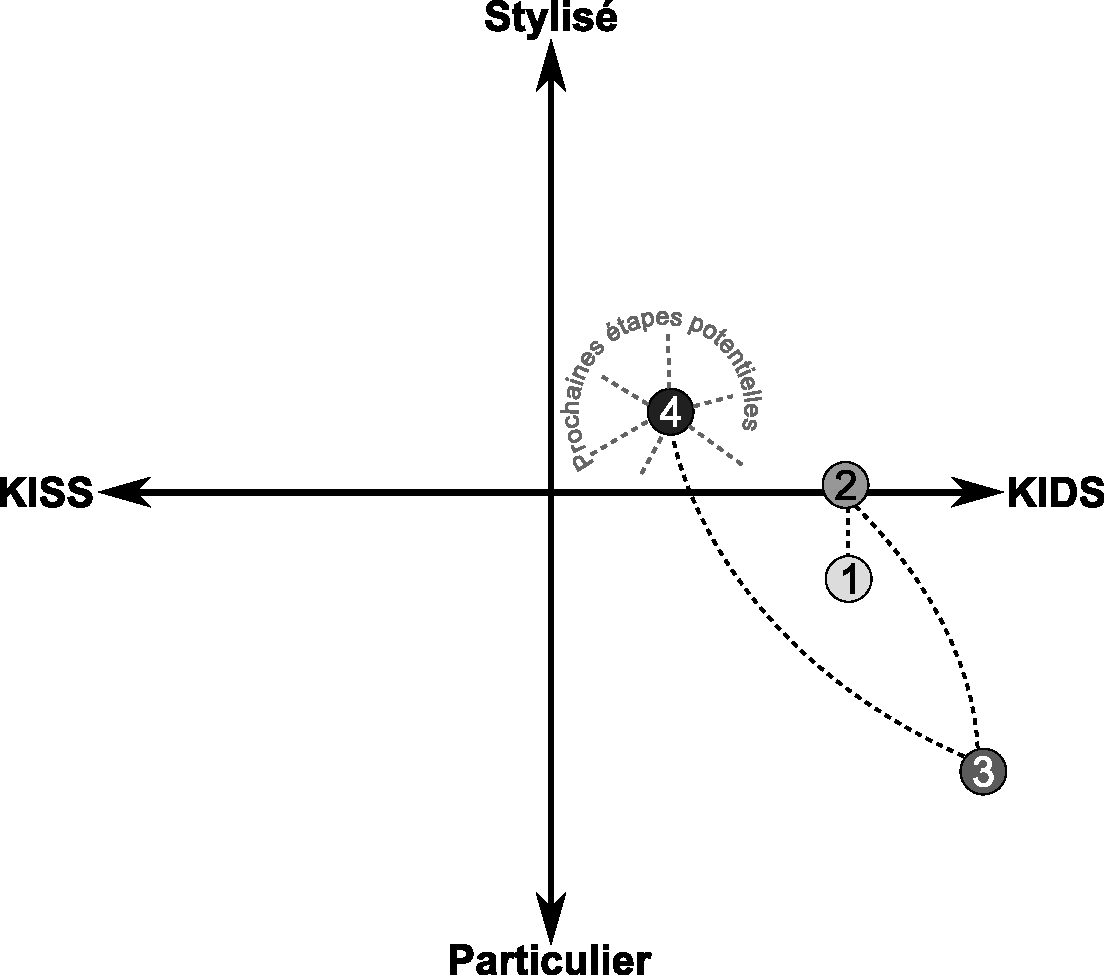
\includegraphics[width=.8\linewidth]{img/trajectoire_simfeodal.pdf}
	\caption[La trajectoire du modèle \simfeodal{}, dans le \og fer à cheval\fg{} de \textcite{banos2013modeliser}.]{La trajectoire du modèle \simfeodal{}, dans le \og fer à cheval\fg{} de \textcite{banos2013modeliser}.\\
	\textit{N.B.: cette trajectoire correspond à la position des mécanismes liés aux seigneurs dans le modèle.}}
	\label{fig:trajectoire-simfeodal}
\end{figure}


Il me semble que ces deux éléments peuvent s'expliquer par la nature de \simfeodal{} et de sa co-construction, qui sont plus exploratoires et abductives que véritablement descriptives.
En témoignent les allers-retours fréquents entre augmentation et diminution de la complexité (axe KISS-KIDS) dans l'historique de développement du modèle.
Une partie de ces évolutions sont prévues dans la démarche KIDS \autocite{edmonds_kiss_2005}, qui débute par un modèle \og complexe\fg{}, descriptif, qui sera ensuite progressivement simplifié si cela n'en diminue pas l'utilité.
La \og simplification\fg{} de \simfeodal{} s'inscrit dans cette démarche.
La complexification de certains agents et mécanismes va pourtant à l'encontre de cette logique, et a posteriori, j'aurais tendance à ne caractériser \simfeodal{} que comme un modèle exploratoire, sans le positionner uniquement sur l'axe KISS-KIDS, sinon en explicitant qu'il s'inscrit au départ dans un positionnement descriptif dont on a ensuite accepté de réduire la complexité.

Ce sont avant tout les envies du groupe de travail qui guident le développement du modèle, influencées par les résultats successifs du modèle et par leur exploration.
Ces envies varient, s'accompagnent d'abandon de questionnements initiaux et de nouvelles questions, évoluant parfois en sens inverse des choix passés, voire correspondant à de véritables \og retours en arrière\fg{} comme dans le cas des lignages seigneuriaux, abandonnés après avoir été très spécifiés.
La forme irrégulière de la trajectoire de \simfeodal{} peut interroger de prime abord, mais résulte en fait des multiples interactions entre les concepteurs du modèle et n'est que la matérialisation du processus abductif qui a guidé la co-construction de \simfeodal{}.

\subsection{Conclusion : Modéliser avec et pour les autres.}

Dans cette sous-partie nous avons montré que le modèle, en tant qu'outil informatique, a davantage constitué un support à la discussion interdisciplinaire et à l'explicitation des hypothèses et connaissances qu'à seulement évaluer la capacité de ces hypothèses à reproduire les dynamiques empiriques de polarisation, de hiérarchisation et de fixation du peuplement.
La construction de \simfeodal{} n'a pas été transdisciplinaire :
	tous les participants n'ont pas également contribué à toutes les tâches de modélisation.
Au contraire, la vision interdisciplinaire souhaitée initialement a été conservée, dans le sens où les connaissances et compétences propres de chacun des participants ont été mutualisées pour les tâches qui y correspondaient le mieux.
De la même manière qu'on ne peut acquérir une connaissance thématique approfondie d'un sujet complètement inconnu en quelques années, on ne peut pas non plus y acquérir les compétences techniques avancées nécessaires à l'implémentation de modèles de simulation complexes et détaillés.

Pour autant, je crois qu'on peut tout de même caractériser cette construction interdisciplinaire et collective comme une co-construction, car chacun est intervenu sur chacune des étapes de la construction et de l'évaluation du modèle.
Il résulte de cette co-construction un modèle à la trajectoire irrégulière, faite de fréquents allers-retours, et au positionnement final difficile à caractériser dans des référentiels existants autocite{banos2013modeliser} tant ses composantes sont hétérogènes.
Cette trajectoire particulière me semble inhérente au mode de co-construction, résolument exploratoire et à but heuristique qui a été collectivement choisi et mis en oeuvre.

La satisfaction collective qui ressort de cette expérience de modélisation me paraît due à des facteurs individuels autant que collectifs.
Individuellement, chacun a voulu s'inscrire pleinement dans cette expérience interdisciplinaire et a accepté de passer outre ses habitudes disciplinaires.
Collectivement, c'est le choix d'une organisation horizontale, bâtie sur un temps long de plusieurs années autour des complémentarités de pratiques et de connaissances, qui a permis à ce projet d'aboutir.

\section*{Conclusion}
\addcontentsline{toc}{section}{\protect\numberline{}Conclusion}

Ce chapitre a présenté deux retours réflexifs, assez isolés au premier regard, sur la spécificité de l'exploration de données de simulation et sur les modalités du processus de co-construction mis en œuvre dans le cadre de la construction et de l'évaluation de \simfeodal{}.
Chacune de ces sous-parties a déjà donné lieu à une conclusion intermédiaire, et je ne reviendrai ici que sur leur complémentarité.

Que ce soit sur le plan méthodologique de l'exploration de données issues de simulation, ou sur le plan conceptuel de la construction de modèle, l'élaboration d'une démarche exploratoire, faite d'allers-retours entre la conception et l'évaluation, entre la visualisation et l'implémentation, ressort comme un moyen fonctionnel de favoriser l'interdisciplinarité.
Cette démarche peut pour cela être bâtie autour d'un objet commun -- car partagé -- et positionné à l'interface entre les disciplines.
L'objet commun que constitue le modèle et les données qu'il produit permettent de faire en sorte que le processus de modélisation ne soit pas qu'une expérience de pensée.
Cet objet matérialisé, parce qu'il peut être exploré, guide l'expérience collective et constitue ainsi une interface commune, support au dialogue entre des chercheurs venant de différentes disciplines, en laissant l'exploration guider ce dialogue.

C'est en cela que la démarche mise en place autour de la construction et de l'évaluation peut être considérée comme facilitant la \og mise en situation d'étonnement\fg{} \autocite[241]{banos2005voie}.
L'exploration des hypothèses thématiques, par le modèle, et du modèle, par ses sorties, stimulent ainsi le cheminement abductif qui permet de dépasser les \textit{a priori} et implicites disciplinaires et d'aboutir à la réalisation d'un modèle utile à tous ses concepteurs.